\documentclass[12pt, twoside, titlepage]{book}

\title{Visualizing laser scanner point clouds as 3d panorama}
\author{Adam Kalisz}
\date{July 2015}


\usepackage[style=alphabetic,backend=biber,sorting=none]{biblatex}
\addbibresource{references.bib}
%For (accessed) info
\DefineBibliographyStrings{english}{%
	urlseen = {Retrieved},
}

\usepackage[utf8]{inputenc}
\usepackage[T1]{fontenc}
\usepackage{graphicx}
\graphicspath{{images/}}
\usepackage[a4paper, width=150mm,top=25mm, bottom=25mm, bindingoffset=6mm]{geometry}

\usepackage{caption}
\usepackage{subcaption}


\usepackage{fancyhdr}
\pagestyle{fancy}
\fancyhead{}
\fancyhead[RO, LE]{Visualizing laser scanner point clouds as 3d panorama}
\fancyfoot{}
\fancyfoot[LE, RO]{\thepage}
\fancyfoot[LO, CE]{Chapter \thechapter}
\fancyfoot[CO, RE]{Adam Kalisz}
\renewcommand{\headrulewidth}{0.4pt}
\renewcommand{\footrulewidth}{0.4pt}

\usepackage{pgfgantt}


\begin{document}
	
	\begin{titlepage}
	\begin{center}
		\vspace*{1cm}
		
		\Huge
		\textbf{Visualization of laser scanner point clouds as 3D panorama}
		
		\vspace{0.5cm}
		\Large
		Using laser scanning to reconstruct the facade of the Pellerhaus Nürnberg in its historic state
		
		\normalsize
		\vspace{1.5cm}
		
		\textbf{By}\\
		\vspace{0.5cm}
		\textbf{Adam Kalisz}\\
		\textbf{2265000}\\
		
		\vspace{1.5cm}
				
		
		A thesis presented for the degree of\\
		Bachelor in Media Engineering
		
		\vfill
		
		\vspace{0.8cm}
		
		{
\includegraphics[width=0.7\textwidth]{TH_Nuernberg_Logo.png}}
		
		\Large
		\normalsize
		Elektrotechnik Feinwerkmechanik Informationstechnik\\
		Georg-Simon-Ohm Technische Hochschule Nürnberg\\
	
		\vfill
		
		\vspace{0.8cm}
		Thesis advisors:\\
		Prof. Dr. Stefan Röttger\\
		Prof. Dr. (USA) Ralph Lano\\	
		\vspace{0.8cm}
		
		Submission date:\\
		July 15th, 2015
		
		\vspace{0.8cm}
		
		Location:\\
		Nuremberg, Germany
		
		\vspace{0.8cm}
		
		Keywords:\\
		LiDAR, point, cloud, laser, scanning, panorama, Blender
		
		
		
		
	\end{center}
\end{titlepage}
	
	\thispagestyle{empty}
	
	\thispagestyle{plain}
\begin{center}
	
	\LARGE
	\textbf{Declaration}
	
\end{center}
\vspace{100pt}
\underline{\textbf{Plagiarism Declaration in Accordance with Examination Rules}}
\vspace{12mm}

I herewith declare that I worked on this thesis independently. Furthermore, it was not submitted to any other examining committee. All sources and aids used in this thesis, including literal and analogous citations, have been identified.


\newcommand*{\Overlined}[1]{%
	\par\noindent\makebox[2.5in]{\hrulefill}%
	\par\noindent\makebox[2.5in][l]{#1}%
}%


\begin{flushleft}
\vspace{12mm}
\Overlined{Signature}

\end{flushleft}

	\thispagestyle{plain}
\begin{center}
	
	\LARGE
	\textbf{Abstract}
	
\end{center}
\vspace{100pt}

This study examines a novel approach to convert point clouds generated via laser scanning into textured 3D-meshes. The title of this paper is "Visualization of laser scanner point clouds as 3D panorama".
The approach is field-tested with a use case scenario where the interested reader will learn about our research on the 3D-model reconstruction of the historic Pellerhaus in Nuremberg, Germany, as it looked before its destruction during World War II.\\

The motivation behind the report, details about the project and existing solutions for creating virtual reconstructions are introduced in Chapter One.
The background research that provided necessary fundamentals to start the project, for example how the Pellerhaus evolved or what exactly a 3D panorama is, is described in the second chapter.
The third chapter presents the development process of the software tools applied to achieve the goal of reconstructing historic 3D models from various data, such as images and laser scans. To accomplish this, a custom converter software was written, which reads point cloud files and outputs the meshed and textured 3D-object file. The working title of this software is "PointCloud2Blender", \textit{PC2B} in short.
As a real world use case the creation of a photorealistic three-dimensional mesh from laser scans via LIDAR devices is described in detail in Chapter Four.
Chapter Five concludes the work and presents future work. It contains the results, failures, and successes of this research. Furthermore, it discusses different possible ways to build upon the fundamental insights gained from this report.\\

Due to our modern open culture with several open software, hardware and movie projects - mainly inspired by the Blender Foundation - this research is being made available to the public. During the time of the writing of this thesis the progress is published online at http://bachelor.kalisz.co.

	\thispagestyle{plain}
\begin{center}
	
	\LARGE
	\textbf{Acknowledgements}
	
\end{center}
\vspace{100pt}

This research could not have been performed without the assistance, patience, and support of many individuals.\\

On behalf of the historical expertise required for this research, I would like to thank the Geschichtsarchiv Langwasser, including Mrs Edith Schroth and Mr Alfred Schroth for their constant support in providing old photographs, material and making contact to various institutions like archives, museums and companies. They initiated the contact with the Altstadtfreunde Nürnberg e.V. as well.\\
Therefore I would like to thank the Altstadtfreunde Nürnberg e.V. for a huge amount of historic pictures and professional guidance regarding the history of the Pellerhaus. I am happy to get the opportunity to be supported by chairman Mr. Karl-Heinz Enderle during my research.\\

Secondly, I have to thank my thesis advisor, Mr. Prof. Dr. Stefan Röttger for mentoring me during my undergraduate studies. Not only did he prove his confidence in me by encouraging me to teach computer graphics to other students by letting me demonstrate how much fun it can be creating graphics with the open source 3D graphics suite Blender and offered me several jobs in 3d animation. His insight lead to the initial proposal to examine the possibility of reconstructing the Pellerhaus facade. In addition I would like to extend my gratitude to Mr. Prof. Dr. (USA) Ralph Lano for supervision during my studies. His teaching style and enthusiasm made a strong impression on me and I have always carried positive memories of the classes I attended. Although, the classes I took have not been mandatory and rather seldom they made a lot of fun (e.g. XBox programming with Unity), he was always very helpful and friendly. I would like to thank you very much for your support and understanding over these past four years.\\

Finally I would like to extend my deepest gratitude to my family without whose love, support and understanding I could never have completed this bachelor's degree.


	\tableofcontents
	
	\listoffigures
	\listoftables
	
	\chapter{Introduction}
	In this chapter we introduce the project by providing a broad overview of the reason why this topic has been chosen, consideration of various state-of-the-art technologies available for executing the research and the definition what result we expect to get from this report.

\section{Motivation}

The field of 3D computer graphics has always been a fascinating subject to me. Creating virtual worlds and being able to inspect those from every possible viewpoint is a great way to present almost any object one can think of to a wider audience. I finished my apprenticeship as a A/V media designer, so computer graphics are a helpful tool to e.g. previsualize camera work. The best fact about 3D is that it has so many versatile applications in many fields. 3D information can be retrieved from 2D images, taken with a real photo camera, via photogrammetry and can, in turn, be rendered onto a flat computer screen by rendering a three-dimensional scene with a virtual camera. At the point a object is available as a 3D model, it can be postprocessed in various ways. It can be animated, physically simulated and eventually rendered as a video. With modern display technologies the movie can be played out as a stereoscopic one and viewed with anaglyph (red, cyan), polarized, shutter or even without glasses by using e.g. a parallax barrier display (Wikipedia, \parencite{wiki:ParallaxBarrier}). Furthermore objects can become tangible via 3D printing or can be inspected interactively in games with the help of virtual reality glasses like the Oculus Rift (Oculus VR, \parencite{OculusVR}). It is amazing that anyone can create and enjoy those virtual worlds today.

Additionally, I am highly interested in historical topics. As an active member of a local citizens association and representative of a settlement, where I am always available for any citizenship matters that people might have, I get to know many interesting people and the projects they are working on. Thus I am learning a lot about interesting historical facts and development of culture. Of course, not only about positive history. Especially the history of the place where I live, Langwasser, district of Nuremberg, Germany, is very terrifying and shocking. The district has been formerly used for tent cities and the Märzfeld ("March Field", a representation and parade ground) during the Reich Party Congress in Nuremburg, Germany, between 1933 and 1938 (Wikipedia, \parencite{wiki:NaziPartyRallyGround}). The construction of a railway station, called Bahnhof Märzfeld which is located right in the center of Langwasser, was partly finished in 1938. That station has been used initially to transport the members of the Reich Party Congress to the event. During World War II it was used for the deportation of about 940 people to concentration camps, where only 17 of them survived (Stadtteilforum Langwasser, \parencite{StadtteilforumTafel6}). This railway station is in a ruinous condition at the moment. People go by without noticing that this is real history that passes them by. This was a big concern for me, so I started to search for ways to present history in a modern way, making it educational on the one hand and enjoyable on the other hand.

Consequently, there was the day I talked to my professor, Mr. Dr. Stefan Röttger, about my wish to use laser scanning for historic 3D reconstruction. Suprisingly my professor told me, that we have a laser scanning device at university which could be used for a thesis. The moment he told me that, was the moment I made my decision to center my thesis around laser scanning.

Lastly, a strong motivational force was discovered after researching how the laser scanner point cloud can be used to create the historic building model based off of a recent laser scan. 3D software enables a user to tweak automatically generated meshes or even to add new geometry. Due to my personal experience with the open source 3D graphics suite Blender and the decreasing interest in other software like Autodesk 3ds Max or Maya in favor of Blender (Google Trends, \parencite{Interest3DSoftware}) I decided to use Blender for the 3D modeling and animation part of this research. According to the trend it is a better option since it is being used by a greater number of artists and therefore future work will be of help to a lot of people. In addition, the source code of Blender is open. Any research based on it might benefit other researchers due to its open nature. Inspired by the Blender Foundation, I wish to make my work available to the public as much as possible during and after the research. Every person should have the right to learn from the findings in my report. As a result, it was necessary to be able to work with laser scanner output, namely point clouds, in Blender. Unfortunately Blender is not designed to work with point clouds at the time of this writing. This research should adress this issue by providing a way to complete the laser scanning production pipeline for artists who want to use Blender, though not exklusively!

As will be described in greater detail hereafter, the aforementioned facts lead to an initial project specification. 

\section{Initial project specification}

The idea for this research started with the personal concern of reconstructing a historical site like the old railway station in Langwasser in its historic state. Due to the fact that this railway station has never been fully finished and therefore poor historical documentation, a 3D reconstruction wouldn't be complete. Luckily the famous Pellerhaus was the perfect candidate for this research\footnote{Amount of historical photos: Bahnhof Märzfeld: 9; Pellerhaus Nürnberg: 190}. After its destruction during World War II, it was rebuilt quite differently to the original state. While the inner courtyard is almost finished with reconstruction at the time of this writing, the facade is still looking modern. At that point, it was clear that the main research topic is going to examine ways to reconstruct the Pellerhaus facade in its historic state.
A more concrete specification was defined by considering how this is going to be done. The current state of the building has to be captured with laser scanning technology to get the correct measurements from the real world reference. We use a FARO Laser Scanner Focus\textsuperscript{3D} X Series device for this project.
This point cloud data needs to be processed then. To do so, a custom software is required to be written, which can read a file format exported from the proprietary FARO SCENE application, create a panoramic image representation of the data, use it to generate a 3D mesh surface and export this mesh to a widely supported file format. This research will mostly rely on the open source software Blender to model and animate the historic state of the Pellerhaus, thus it is crucial to provide a compatible output to be used as a basis for the design process. By creating a textured surface from the point samples, this research will provide a way for the artist to overcome a bad design decision in Blender, which is making it not capable of displaying or rendering colored point clouds at all (see thread by author on BlenderArtists \parencite{webBlenderArtistsPointCloudSupport} ). The goal of this research is to get a 3D model of the Pellerhaus in its historic state from 1605 by utilizing point clouds generated via laser scanning as described before.

\section{Project schedule}

This project is divided into two main phases. The first phase is developing the software for converting laser scanner point clouds as 3D panorama meshes. The second one is designing the historic 3D model from this initial mesh.\\

This is visualized in the following GANTT chart:\\

\definecolor{RoyalBlue}{RGB}{92,102,149}
\definecolor{OliveGreen}{RGB}{51,151,102}
\definecolor{Maroon}{RGB}{180,20,53}
\begin{ganttchart}[
	x unit=1.3cm,
	y unit title=0.7cm,
	y unit chart=0.8cm,
	vgrid, hgrid,
	time slot format=isodate-yearmonth,
	compress calendar,
	title/.append style={draw=none, fill=RoyalBlue!50!black},
	title label font=\sffamily\bfseries\color{white},
	title label node/.append style={below=-1.6ex},
	title left shift=.05,
	title right shift=-.05,
	title height=1,
	bar/.append style={draw=none, fill=OliveGreen!75},
	bar height=.6,
	bar label font=\normalsize\color{black!50},
	group right shift=0,
	group top shift=.6,
	group height=.3,
	group peaks height=.2,
	bar incomplete/.append style={fill=Maroon}
	]{2015-01}{2015-07}
	\gantttitlecalendar{year, month=shortname} \\
	
	\ganttset{progress label text={}, link/.style={black, -to}}
	\ganttbar[progress=100, name=pp]{Laser Scanning}{2015-01-15}{2015-01-25} \\
	
	\ganttgroup{Software development}{2015-02-15}{2015-06-10} \\
	\ganttbar[progress=100, name=T1A]{Import}{2015-02-15}{2015-02-18} \\
	\ganttbar[progress=100]{Processing}{2015-02-19}{2015-03-25} \\
	\ganttbar[progress=100, name=T1C]{Export}{2015-03-24}{2015-04-01} \\
	\ganttbar[progress=100]{Testing / Bugfixing}{2015-02-26}{2015-06-10} \\
	
	\ganttgroup{Video production}{2015-06-08}{2015-07-10} \\
	\ganttbar[progress=100, name=T2A]{Modeling}{2015-06-08}{2015-06-10} \\
	\ganttbar[progress=100]{Animation}{2015-06-10}{2015-07-02} \\
	\ganttbar[progress=100]{Rendering}{2015-06-12}{2015-07-10} \\
	
	\ganttset{link/.style={OliveGreen}}
	\ganttlink[link mid=.4]{pp}{T1A}
	\ganttlink[link mid=.159]{T1C}{T2A}
	\label{tab:project_schedule}
\end{ganttchart}\\


\section{State-of-the-art methods for 3D reconstruction}

There are several methods that allow for the generation of 3D meshes from various data. One can either use several still images or videos, sample the real world with modern sensor technology or use open data for generating geometry of varying complexity. This is described as follows:

\subsection{Light Detection And Ranging (LiDAR)}

The term Light Detection And Ranging (in short LiDAR) is commonly used with high precision applications, such as scanning and mapping of indoor and outdoor environments. It uses a laser beam emitter and receiver. By using the Distance-Speed-Time formula it is very easy to compute how far away an object is:\\

$$  speed = \dfrac{distance}{time} \Longleftrightarrow distance = time * speed $$\\
The time between sending a signal and receiving it is measured and multiplied by the speed of light ($c = 299,792,458 \medspace \frac{m}{s}$, Wikipedia \parencite{wiki:SpeedOfLight}). This returns the meters the light traveled from the emitter to the obstacle and back. Dividing this distance by two yields the range to the obstacle in meters (Schroeder \parencite[see][p8-9]{dp_lidar}).

As this gives the meters to only one specific point, it is necessary to keep measuring from different view orientations. This can be done by rotating the scanning device horizontally and vertically simultaneously. To avoid mechanical imprecision or cables from winding up most devices usually use one motor for the horizontal and another motor to control a flat mirror on an elliptical mount for the vertical rotation. That way it is possible to sample a lot of points around the device position quickly and effectively.

\begin{figure}[h]
	\centering
	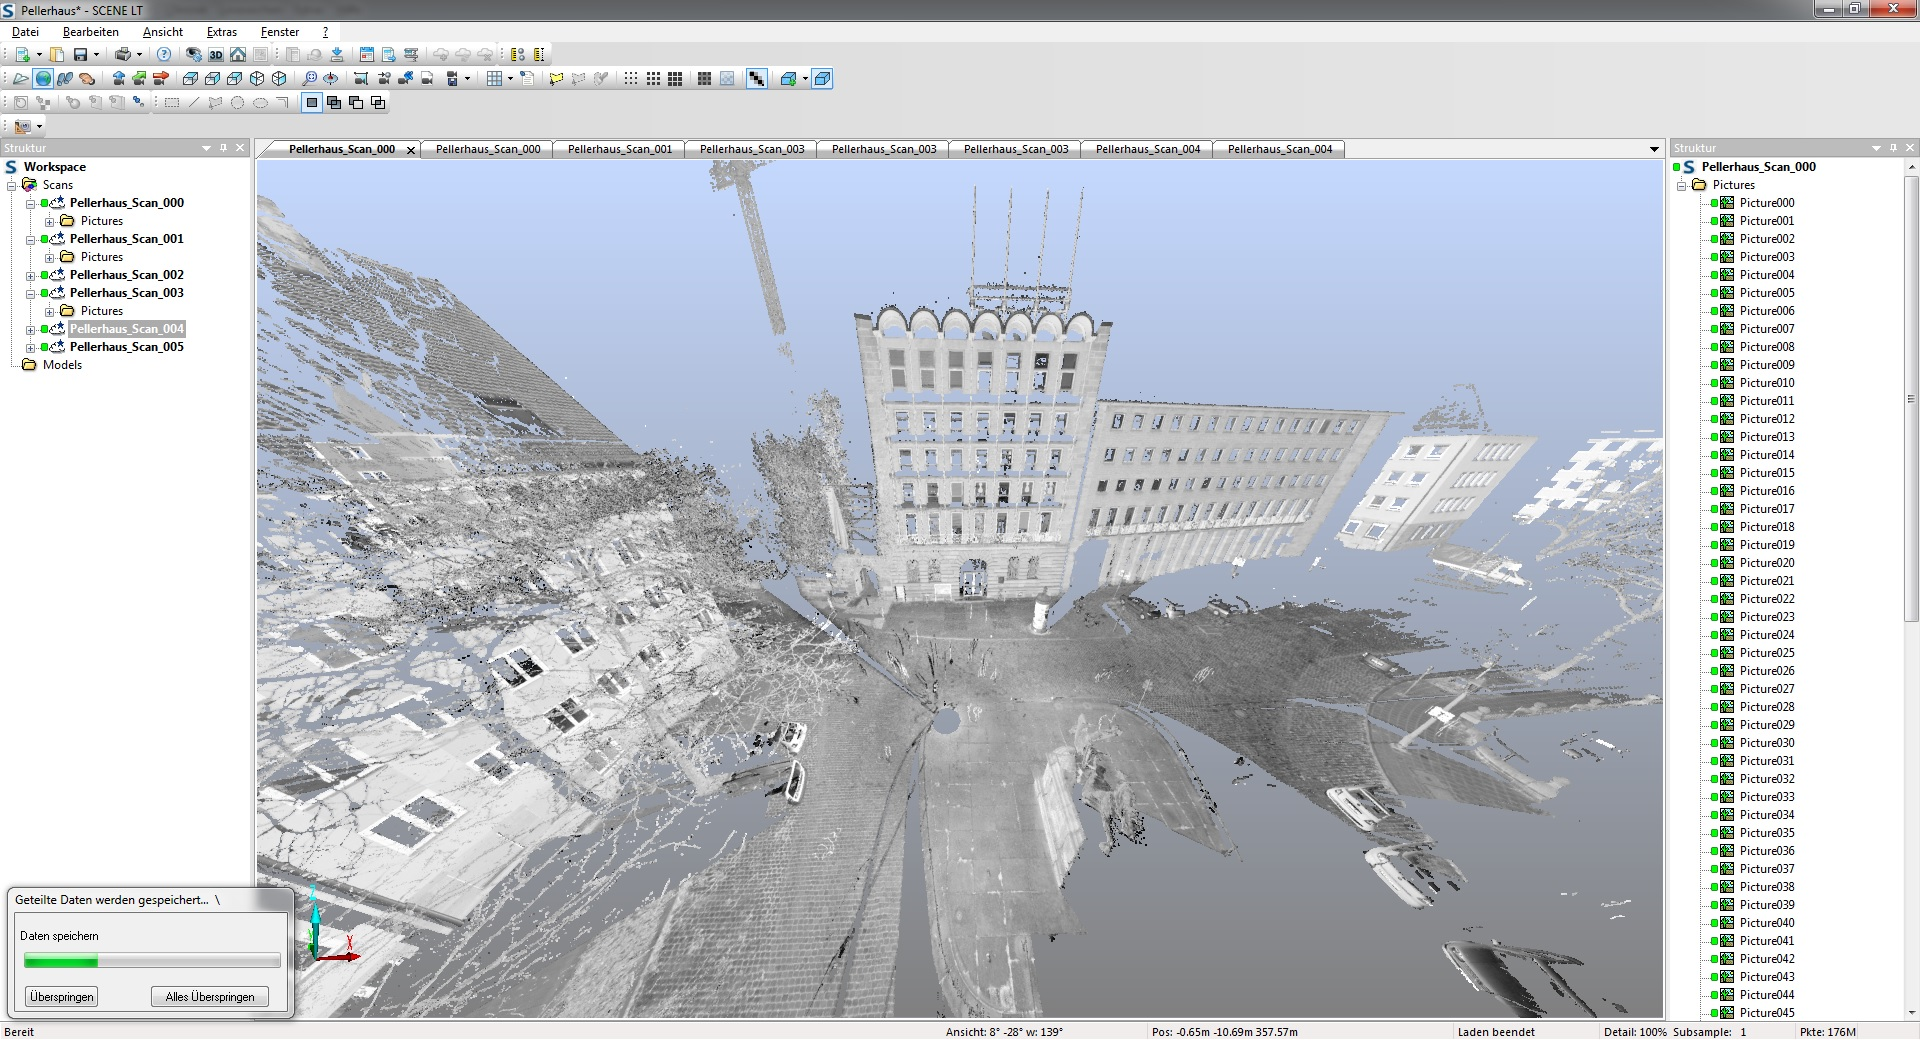
\includegraphics[scale=0.25]{Pellerhaus_FirstGlance.jpg}
	\caption{LiDAR Scanner Point Cloud of the Pellerhaus}
	\label{fig:LiDAR_PointCloud}
\end{figure}

In this work the LiDAR scanner FARO Focus\textsuperscript{3D} is being used. It is capable of capturing 976,000 points per second with a vertical and horizontal field of view of 305 and 360 degrees, respectively (Techsheet FARO Focus\textsuperscript{3D}, \parencite{faro_techsheet}). For allowing a better registration additional sensors can be used such as GPS for localization and a barometer for height measurement. The measured points can be colored using an automatic color overlay from a built-in camera at a 70 megapixel resolution. The price for the Focus\textsuperscript{3D} totals at 61,404.37 Euro (Opti-cal Survey Equipment Ltd. \parencite{survey_equipment}).

Besides using a stationary device, portable devices are also available. Recently a new technology has been revealed by Csiro and is called \textit{Zebedee}. This handheld laser scanner can be used in challenging environments where a stationary device would require several scans to cover the whole area (e.g. caves, staircases) while the operator is walking. It samples over 40,000 range measurements every second and consists of a 2D laser scanner mounted on a spring system (Mail Online, \parencite{zebedee_info}). Especially the visual effects field has a great use for this device, since the environments can vary a lot during video shootings and a 3D mesh representation is ubiquitous today. The price for the ZEB1 handheld laser scanner is 17,000 Euro\footnote{Source: Personal contact to sales team}.

Although measuring with laser technology can be found in household devices as an alternative for tape measuring, it is still quite complicated to reverse engineer such devices to get the raw distance reading. Fortunately a group of engineers tried to bridge the gap by starting a crowd funding campaign for a low-cost laser range finder, called the LiDAR-Lite (PulsedLight \parencite{pulsedlight}). It has a total range of 40 meters with a resolution of 1 cm. During this research this sensor is being used with a custom arduino build to examine how it can be used as a cheap alternative to the examples mentioned in the beginning. The price for one module is at 82 Euro.

\subsection{Ultrasonic}

In contrast to LiDAR, most ultrasonic sensors are cheap, but generally are not used for higher distances at several tens of meters (though, there are products for a range higher than 100 meters, compare VEGAPULS 69 \parencite{vegapuls}). The reason for this is that sound is usually affected stronger by environmental properties than light (compare Sensors Magazine \parencite{sensorsmag}). Due to this they are often used for shorter distances e.g. for near field obstacle recognition in robotics or in small desktop laser scanners (compare Dinh \parencite{yt_smalldesktoplaser}). Typical ultrasonic sensor modules with a maximum range of around 5 m can be purchased for 5 Euro already.



\subsection{Photogrammetry}

Photogrammetry (also referred to as multi-view reconstruction) is a technique from the Computer Vision field and presents a cost-effective alternative to laser scanning. A real 3D object can be reconstructed as a virtual 3D model by using photographs of the scene and feeding them into such software. This works by detecting image features (for example by using Harris Corner Detector or SIFT algorithms), matching those between image pairs, computing the respective camera positions and re-projecting the reconstructed 3D points to get a point cloud representation of the real photograph (compare Solem \parencite[][p29]{bookProgrammingComputerVisionwithPython}).
The Computer Vision algorithms get better each day and there is plenty of software using them. Basically we can distinguish between open source, free or commercial software for this task. Usually open source software can be free to use, too. Though, it might have some limitations defined by its license, e.g. only granting non-commercial use. On the contrary, some licenses even allow users to sell the software under a different brand name as is the case with e.g. Blender. In this example the GNU GPL Version 3 license allows a company to sell Blender with prices starting at 47 Dollar. As this is only a side note, more information on that topic can be found in \parencite{blender_rebranding}.
To compare the results of open source and commercial photogrammetry software we processed 356 photos of the Pellerhaus with two applications. On the one hand VisualSFM for generating a sparse point cloud in conjunction with CMP-MVS for the dense point cloud generation via open source tools have been used. On the other hand the commercial software Agisoft Photoscan Professional was used which costs 3,499 Dollars but can be tested with a fully functional 30 day trial, like in this research.

\begin{figure}[h]
	\centering
	\begin{subfigure}[b]{1.0\textwidth}
		\centering
		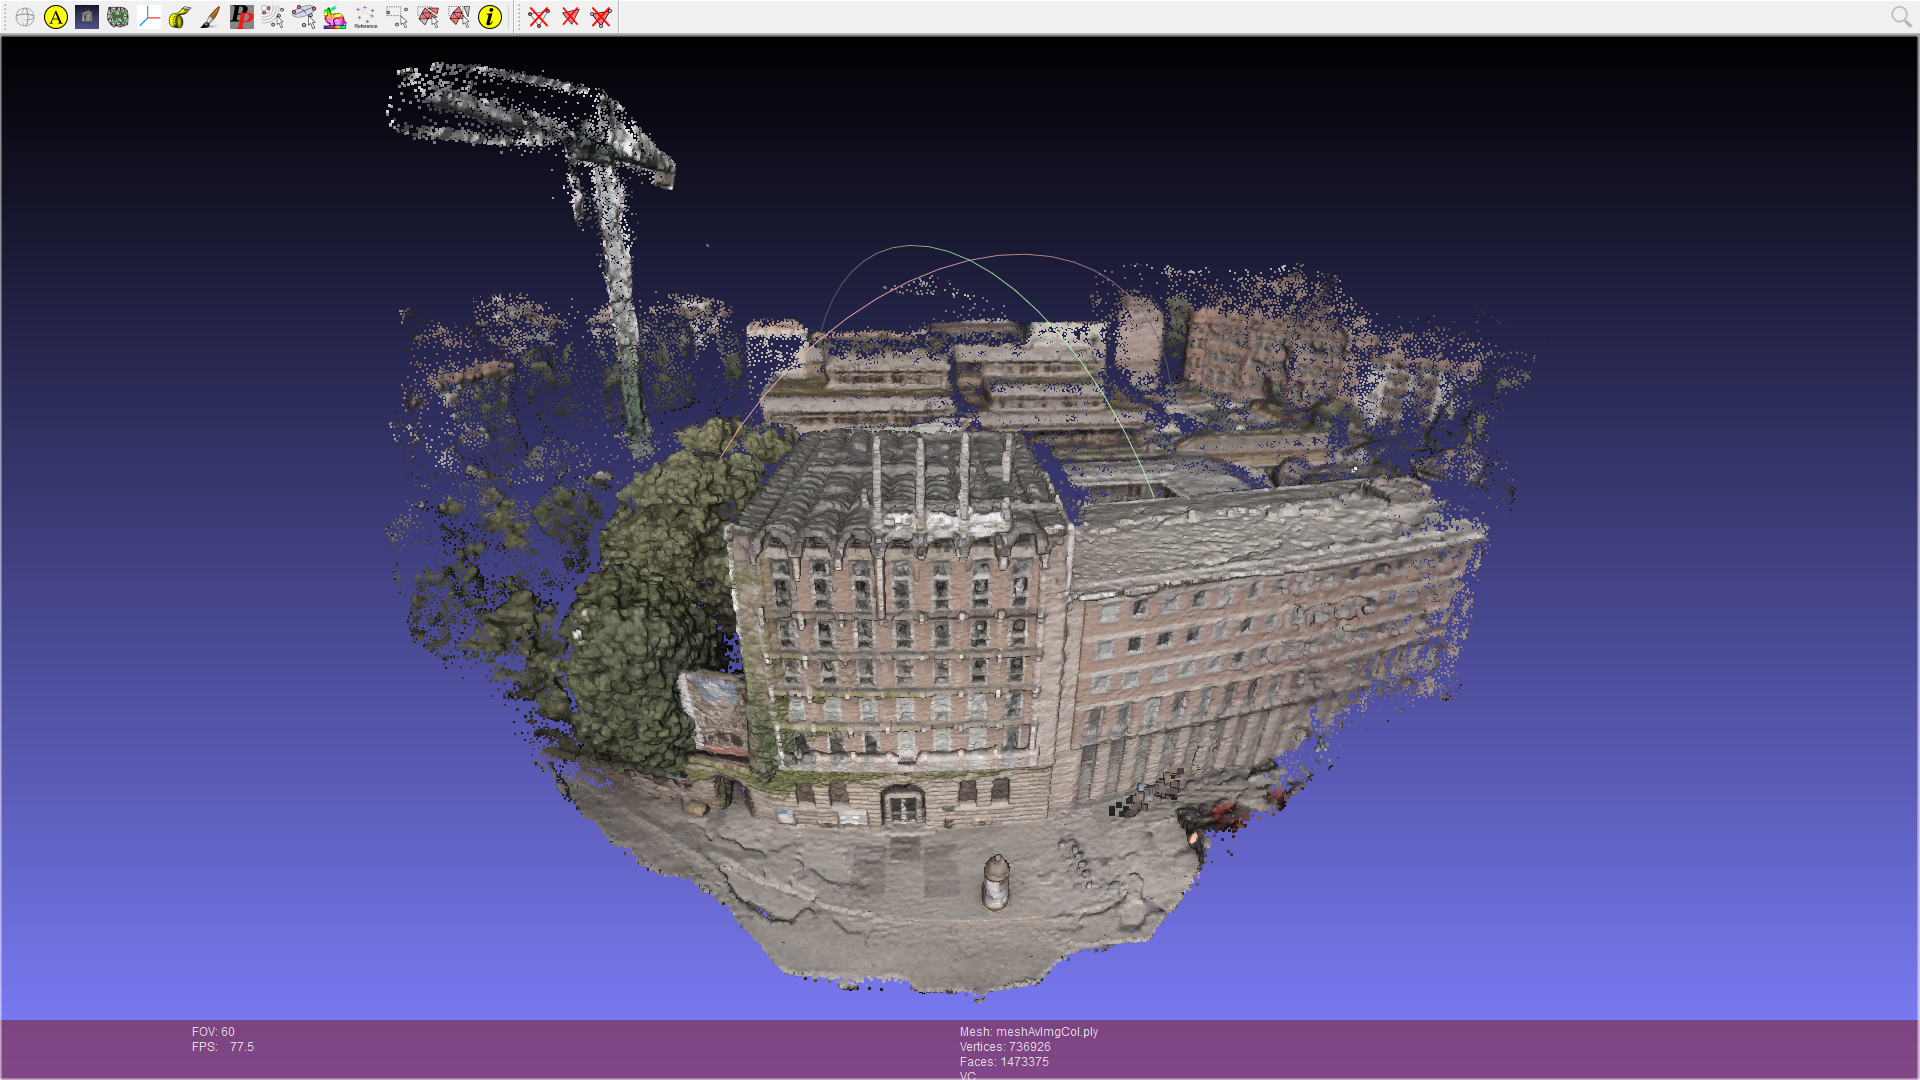
\includegraphics[width=\textwidth]{Photogrammetry_VisualSFM.jpg}
		\caption{Open Source: Visual SFM + CMP-MVS (736,926 points)}
		\label{fig:visualsfm}
	\end{subfigure}
	\hfill
	\begin{subfigure}[b]{1.0\textwidth}
		\centering
		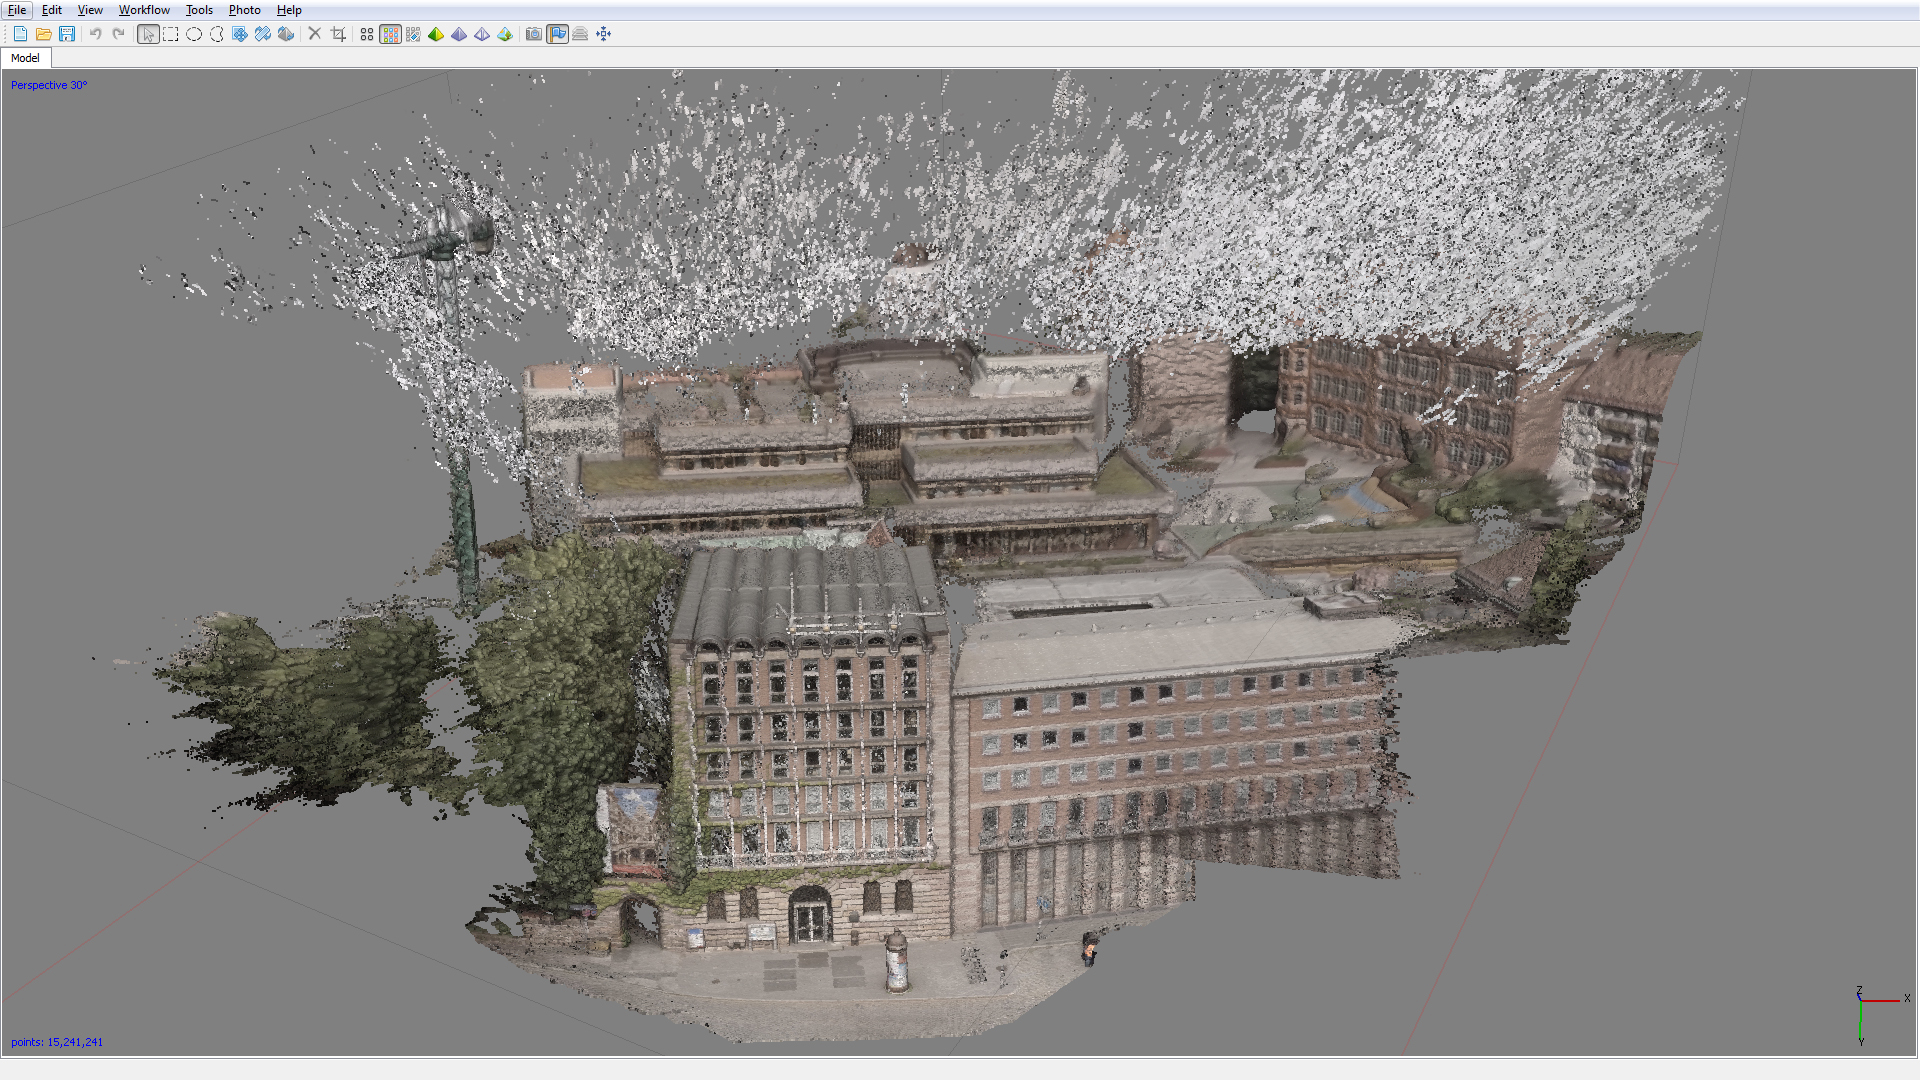
\includegraphics[width=\textwidth]{Photogrammetry_Agisoft.jpg}
		\caption{Commercial: Agisoft Photoscan (15,241,241 points)}
		\label{fig:photoscan}
	\end{subfigure}
	\caption{Multi-view reconstruction point clouds generated from 356 photos}
	\label{fig:multiview reconstruction pellerhaus}
\end{figure}

Comparing the results, the point cloud output from Agisoft Photoscan is much more detailed, approximately by a factor of 20. Furthermore VisualSFM created a bent facade, whereas Photoscan preserved all important straight lines. All in all it can be observed that the algorithms of Photoscan are more sophisticated and suited better for images taken with a great amount of lens distortion, though this is something that should be avoided when considering using the footage for multi-view reconstruction (see Balletti et al. \parencite{calibration_of_action_cameras}). Both applications generate a model that can provide a good initial mesh of a scene, but the computation takes very long. Photoscan was using all ressources of an eight core Intel i7 workstation with 16 of RAM running for about 4 days.

Photogrammetry will be used in this project to try reconstructing surfaces from historical images. Fortunately historical stereographic image pairs are provided through the Altstadtfreunde Nürnberg e.V. By matching the laser scanner data with the Photogrammetry output a good groundwork is expected to be done for the final surface reconstruction.

\subsection{Depth Cameras}

Instead of using photogrammetry software to retrieve 3D information from images, Depth Cameras can be used which encompass the same functionality in hardware. Popular devices are e.g. the Microsoft Kinect v1 and v2 or the Asus Xtion Pro Live, typically ranging between 100 and 200 Euro. Using stereo matching algorithms those devices can determine the distance, or depth, of a certain point. First, an infrared projector emits a speckle pattern which an infrared camera analyzes to match points between the emitter and projector. By using a mathematical process based on trigonometry called Triangulation (compare Wikipedia \parencite{wiki:Triangulation}) it is possible to calculate the distance to a point if certrain properties are known, such as the distance of a fixed baseline between two observing points and the angle from the baseline to the observed point. There are some problems known with those sensors which limit their use mostly to indoor applications. Direct sunlight can wash out the speckle pattern or multiple sensors can confuse each other. Despite those issues Depth Cameras provide a simple and fast way to get 3D point clouds of real objects. Custom software can be written and access this data directly from the depth sensor. The Microsoft Kinect SDK provides some examples how this can be accomplished and the Kinect Fusion project presents a complete solution for creating 3D surfaces of high resolution in real-time (see Newcombe et al. \parencite{kinectfusion}).

\subsection{Google Maps \textsuperscript{\textregistered} }

The commercial application allows viewing cities from the sky with a rough representation of 3D building shapes (compare Zamora \parencite{google_maps}). While this service had gray boxes some years ago, today the visualization is getting more accurate. Nowadays it is possible to see small details with better modeled and textured buildings.

\subsection{Open Street Map \textsuperscript{\textregistered} }

The open source alternative to the commercial service above offers the basic functions for map viewing and navigation. OpenStreetMap (OSM) offers very detailed access to its data, like boundaries, streets and building footprints. That way it is possible to extract simple building shapes (compare F4 \parencite{f4map}) that can be used in custom software free of charge.

To allow for a better mapping of buildings there are also proposals on an indoor version of OSM (compare OpenStreetMap Wiki \parencite{openstreetmap_wiki}). Having this data available is a helpful asset for various applications such as indoor navigation at railway and subway stations, mobile emergency exit information and robotics.

\subsection{Bavarian State Office for Survey and Geoinformation}

Geodata and city plans are usually provided officially through governmental institutions. They provide various types of data, among others historical aerial photographs, digital elevation models (DEM) and also 3D building shapes. For educational purposes (like i.e. this research) they offer a university discount for the data of 25 percent. A usual dataset without any discounts containing 7580 buildings of Langwasser, district of Nuremberg in Germany, costs 1,158 Euro\footnote{Personal research and contact}.

\subsection{Autonomous mapping with UAV's and SLAM}

Drones, or unmanned aerial vehicles (UAV's), are getting more popular each day. Most of them are also equipped with a camera which allows for taking pictures or videos from viewpoints a human cannot reach easily. More expensive drones have LiDAR systems attached (Shen et. al. \parencite{drones_lidar}) which allow - together with the IMU (Inertial Measuring Unit) and GPS (Global Positioning System) to localize it and map its environment. A popular term for retrieving the current position based on various sensor data while creating a virtual representation of the environment at the same time is Simultaneous Localization And Mapping (SLAM).

\subsection{Manual methods}

If all other methods fail, there is still the chance to get a reconstruction done roughly by taking measurements of real objects with measuring tapes or eyeballing. Loading reference pictures from the front, side and top view into a 3D software can already yield decent results. Furthermore this is the standard way a 3D artist would begin to model a digital human or character that a concept artist provided by sketching those three main views of it. Concept art that is accurate and matches every other view can help a 3D artist to block out the shapes very fast. In certain circumstances it can even be faster than setting up a scanning environment or generate a mesh via photogrammetry, because the generated meshes need to retopolgized (that is, re-modelled with a strong focus on the clean layout of the mesh grid) anyway as soon as they are considered to be e.g. used in animation.

\section{Defining the scope of this research}

Although this work uses a combination of several techniques (briefly presented above), the main focus is put on examination if panoramic projection and meshing of laser scanner point clouds will be an aid for 3D reconstruction or not. This will be evaluated by using the result from the custom converter software in a real world use case of using the generated mesh in the design process.
	\chapter{Background Research}
	
\section{Historical fundamentals}


\subsection{Renaissance}

The Renaissance is a historical period from 14th to 17th century, which started as a cultural movement in Italy in the Late Medieval period and later spread to the rest of Europe. This period is considered as the bridge between Middle Ages and Modern History. Even though the renaissance had a major impact all over Europe, the spread of its principles was not made in an uniform fashion. The word Renaissance, litterally meaning "Rebirth" in French, first appears in English in the 1830s.
The Renaissance is mostly known for the cultural revival of the principles developed in the ancient Greece and Roman Empire. This revival brought a gradual a widespread educational reform.
Renaissance had a major role  in politics, its principles being the base of the conventions of diplomacy. In science, the renaissance brought an increased reliance on observation, rather than superstition.
Even though the renaissance had a major impact in all aspects of life between 14th and 17th century, this historical period is mostly known for the impact it had on arts. The most famous examples are the artistic developments and contributions of such polymaths as Leonardo da Vinci and Michelangelo, who inspired the term "Renaissance man".
The Renaissance started in Italy in the 14th century, under the patronage if powerful, dominant families as Medici. The Fall of the Constantinople at the hands of the Ottoman Turks started a migration of Greek scholars towards west. This scholars brought with them the wisdom and knowledge of the ancient Greece and Rome and spread it though the Italian peninsula, in all the major city states, such as Florence, Venice, Genoa, Bologna, Milan and finally Rome, during the Renaissance papacy.
Renaissance influence was felt in literature, philosophy, art, music, politics, science, religion, and other aspects of intellectual inquiry. Renaissance scholars employed the humanist method in study, and searched for realism and human emotion in art.
Renaissance could be considered as an attempt to study and improve the secular and worldly, both through the revival of ancient ideas and principles, and though new approaches to thoughts.
Another major influence of the Renaissance was felt in the economy. One of the best example could be the banking system pioneered by the Medici family in Florence. While the great states of Europe, France and Spain were absolutist monarchies and ma other states were under direct papal control, the independent city republics of the Italian peninsula took over the capitalist principles developed on the monastic estates, and set off a vast unprecedented commercial revolution and financed the Renaissance.

Renaissance Architecture, is the architecture of the period between 15th and 17th century. This period is characterized by a conscious revival and development of ancient Greek and Roman thought and material culture.
Stylistically, Renaissance architecture followed Gothic architecture and was succeeded by Baroque architecture.

"Renaissance style places emphasis on symmetry, proportion, geometry and the regularity of parts as they are demonstrated in the architecture of classical antiquity and in particular ancient Roman architecture, of which many examples remained. Orderly arrangements of columns, pilasters and lintels, as well as the use of semicircular arches, hemispherical domes, niches and aedicules replaced the more complex proportional systems and irregular profiles of medieval buildings."
Renaissance in Germany
Renaissance arrival in Germany and the Low Countries coincided with the development of the printing press (ca. 1450) and was inspired first by German philosophers and artists such as Albrecht Dürer and Johannes Reuchlin who visited Italy.
In the early Protestant regions of the country, the humanism became closely related with the religious turmoil caused by the Protestant Reformation. Various aspects of this turmoil were frequently depicted in the art and the literature from this period. However, the gothic style and medieval scholastic philosophy remained dominant until the turn of the 16th century. With the rise to power of the Emperor Maximilian I of Habsburg (1493-1519), renaissance became the main trend in the land. The emperor was the first truly Renaissance monarch of the Holy Roman Empire, later known as Holy Empire of the German Nation.
One important early example of renaissance architecture is Landshut Residence. In 1536 Louis X, Duke of Bavaria laid the foundation stone for a new residence in the inner city of Landshut. It was the beginning of German Renaissance style under the architect Bernhard Zwitzel from Augsburg; this palace is today known as the "German building". During a journey to Italy, the duke got inspiration for an additional building, the so called "Italian building", which was constructed from 1537 to 1543 in Italian renaissance style.
Another important example of renaissance architecture in Germany is the Augsburg Town Hall. The Town Hall of Augsburg is the administrative centre of Augsburg, Bavaria, Germany, and one of the most significant secular buildings Convention for the Protection of Cultural Property in the Event of Armed Conflict.
The largest renaissance church north of the Alps is St. Michael's Church in Munich. St. Michael's Church is a Jesuit church built between 1583 and 1597 by Wiliam V, Duke of Bavaria. The style in which this church was built will have an enormous influence on Southern German early Baroque architecture. This church was built as the spiritual center for the Counter Reformation. In order to build the church and the adjoining collage, Duke William had to pull down 87 houses, ignoring the protests of the citizens.
Weser Renaissance is a style formed around river Weser in central Germany. The style is very well preserved in the towns and cities of that region. 
Between the start of the Reformation and the Thirty Years War, the Weser region experienced a construction boom, in which the Weser, playing a significant role in the communication of both trade and ideas, merely defined the north-south extent of a cultural region that stretched westwards to the city of Osnabrück and eastwards as far as Wolfsburg.
Castles, manor houses, town halls, residential dwellings and religious buildings of the Renaissance period have been preserved in unusually high density, because the economy of the region recovered only slowly from the consequences of the Thirty Years War and the means were not available for a baroque transformation such as that which occured to a degree in South Germany.

The Pellerhaus
The Pellerhaus on Egidienplatz 23 in Nuremberg was once considered one of the most magnificent examples of a town house of the German Renaissance achitecture.
The house was commissioned by Martin Peller in 1602 and remained in the possession of the Peller family until 1828. 

During the next 100 years the house changes hands several times until 1929 when is bought by the city of Nuremberg under the mayor Herman Luppe. The acquisition of the house by the city assured a proper maintenance of this historical landmark.
Between 1931 and 1934 the city starts a reconstruction program for Pellerhaus, restoring to the old grandeur the yard and the rear facade. The detailed plans of the rear facade, drawn for this project survive until today.
On January 2nd, 1945, Pellerhaus was destroyed in an ally bombing. In fact a huge part of the city was transformed into a leveled surface by bombing and debris removal. 
The elegant and dignified image of Egidienplatz, is not distorted by the flat-roof building of the City Library built between 1955 and 1957. The new reconstruction project is launched in 1955, only this time it was decided to restore to its former glory only the ground floor. The rest of the building will serve only a pure functional role and serve as a library for many years.
In 2005 a new initiative was launched, to help with the reconstruction of Pellerhaus. This project is still active today.\\
\\

See Wikipedia: \url{http://en.wikipedia.org/wiki/The_Renaissance} 

\subsection{Architects}

\textbf{Wolff, Jakob d. Ä., builder, sculptor, *1546 Bamberg, † 4.4.1612 Nuremberg} \\
Wolff became the city architect of Nuremberg in 1596, where he and his son W. d.J. built the Fleischbrücke. During 1601-05 he took part in the new build of the stronghold Marienberg in Würzburg and in the reconstruction of the Echtertor. His principal work is the Pellerhaus in Nuremberg (1602-07), one of the most noble private properties during the German Renaissance (destroyed in the Second World War; the remaining parts of the arcade court have been included in the modern building)


\textbf{Wolff, Jakob d. J., builder, *1572 Bamberg, † 24.2.1620 Nuremberg} \\
Wolff was the student of his father W. d.Ä., was given the job of a (royal adviser?) city builder in 1605, had the permission from the council to stay in Bayreuth, Frauenaurach and Schwabach and started, influenced by the Dutch and Italian Renaissance, 1616 with the new build of the city hall in Nuremberg, which was finished in 1622 by his brother Hans.

\parencite[translated from German]{bookBayerischeBiographische}


\subsection{Pellerhaus}

Before destruction, the Pellerhaus was one of the main sights of Nuremberg. The architecture seems to be the most honorable performance of the local art of construction. Its inner court was considered the probably most beautiful arcade court.\\
As the city descended into shatters in 1945, there were only a few remains of the Pellerhaus. The front-facing house was rebuilt in a modern form 1957 on top of the reconstructed hall. An enourmous effort was done by complementing the courtyard, it was discontinued 1959, though.\\
Not until 2005, 60 years after the destruction, the Altstadtfreunde took the initiative to continue the former abandoned construction of side wing and rear house facade.\\
With the accurate documentation of the pre-war level it is possible to do those court additions with extraordinary accuracy. October 2008 layed the foundation block of building the courtyard completely via donations.\\
Since then with the well corner, side wings and eastern backyard gallery crucial parts have been able to get restored from the old building.\\
With your donation or by purchasing a symbolic block of stone you can help to make one of the greatest achievements of German Renaissance in its historic state come alive.\\
At the time when the merchant Martin Peller started with building his house in 1602, he also layed the foundation block to what later entered as the most magnificient bourgeois house into the history of art. The notion of building an arcade court was not new in Nuremberg. There have been hundreds of gallery courts in the city. Many of them with tracery breastwork made of stone. Though, the Pellerish courtyard bested everything that has been know at that time:\\
On the two long sides it was flanked by noble three-story arcades, with a clear and symmetric structure, though with a rich and filigreed ornamentation. While skimming along it, ultimately the show façade caught the eye with a glorious gable. Seldom one can find forms of the italian renaissance merged with local sensuous enjoyment in such a happy way. Antique style pillars accompany the individual floors, obelisks stretch up into the sky and still the appearance was entirely different than in Italy. The Pellerhof, as a Middle European counterpart to the wonderful arcade courts of Italy, is an indispensable part of european architecture \parencite[translated from German]{afWiederaufbauDesPellerhofes}.\\\\


\begin{figure}[h]
	\centering
	\begin{subfigure}[b]{0.3\textwidth}
		\centering
		
\includegraphics[width=\textwidth]{graph1.png}
		\caption{$before 1945$}
		\label{fig:pellerhaus_historic}
	\end{subfigure}
	\hfill
	\begin{subfigure}[b]{0.3\textwidth}
		\centering
		
\includegraphics[width=\textwidth]{graph2.png}
		\caption{$Pellerhaus 1945$}
		\label{fig:pellerhaus_destructed}
	\end{subfigure}
	\hfill
	\begin{subfigure}[b]{0.3\textwidth}
		\centering
		
\includegraphics[width=\textwidth]{graph3.png}
		\caption{$after 1945$}
		\label{fig:pellerhaus_modern}
	\end{subfigure}
	\caption{The Evolution of the Pellerhaus}
	\label{fig:pellerhaus_states}
\end{figure}

First reconstruction was finished in 1934.
Destruction in 1945.
1955 beginning of new reconstruction.
1955-1957 reconstruction of the base floor finished, but destruction of the upper floors (storey heights also differ from the original).
1960 End of all reconstructions, though people realized that a full reconstruction might happen
1972/73 Building a secondary school on top of the back-facing house area pretty much killed every hope of reconstruction of the Pellerhaus.
The Pellerhof has groined vault.\parencite{afPellerhausMagazin01} \\\\

The Pellerhaus was bought by the Major of Nuremberg in the year 1929. Reconstruction was estimated to need a budget of a Martin Peller to succeed. It was a real mess. But the city felt responsible to finance the reconstruction at that time and fundamentally restored it from 1931 to 1934. The red facades have been cleared up and new stone details have been redone by hand. The were really careful to keep all of the small details and not to recreate the house according to a recent art period. The Pellerhaus was saved. Ten years later, it was hit by bombs. Though, the former restoration is incredible worthy today. Hundreds of plans and photos document every detail of its facade. Without that documentation a reconstruction would have been extremely difficult today.
Why wasn't the Pellerhaus reconstructed?
After the Second World War it was important to find room for e.g. the city archive and a library. It was almost decided to completely embed the Pellerhaus into the library which was build to the right of it. But there was a certain force within the city that didn't allow that. So in the end, the old style Pellerhaus was combined with a new style to allow experiencing the old state a little.\parencite{afPellerhausMagazin02} \\\\

Right to the Pellerhaus there was a library built in 1955. An old arc was destroyed which was senseless. Only some column bases and capitals were still laying in the inner courtyard and were ready to be build into the southern part of the court. So, all six arcs, the little passage next to the front-facing house and the adjacent facade part of the northern court facade needed to be recreated.
The build process was mainly based on photos and the remains of the western side. Measurements have been extracted by examining the remains. Also profiles and design of capitals and ending stones. Overall Forms were reconstruced with the help of historic photos. New constructions were needed for the differing tracery of balustrade areas. It was a stroke of luck that the historic documentation of the house is extensive. This helped even with differences of geometric correct constructions with the new build. Also the Chörleins are documented well enough to allow for a reconstruction. For example, there is a massively wrong ornamentation of Chörleins at window lintels, sockets, and volutes when comparing the rebuild from 1950 with the original. On the contrary, we are much closer at the renaissance original with our new build.
We can proudly say that with our restored state the two time layers 1605/07 and 1957/59 form a harmonic unit.
From April 2013 we moved newly produced stone blocks and a fully donated arc in the pellerhaus. Once again, we noticed the reckless deviation of any regularity. All of the six arcs have different spans and the alignment of the arcarde row is not straight, but has been – in its old parts – slightly bulged out. Though, this might be due to the bombing destruction, just as the fact that the arc row
doesn't continue horizontally but considerably descends from the front-facing house into the courtyard.
The facades of the buildings in Nuremberg have been painted red with white rectangles some times. The reason for this was that the look of mined stones varied quite a lot. So by painting them the houses had a united look. This color is also called the „Nürnberger Rot“ (Terra Norimbergensis rubra), because it is looking like the local sand stone and the color powder is coming from the rural area of Nuremberg. Unfortunately only a few color remains are left until the reconstruction but it is enough to prove the colorfulness of the facade. After finishing the reconstruction in the courtyard repainting the facades in the „Nürnberger Rot“ would be the right decision.\parencite{afPellerhausMagazin03} \\\\


Nuremberg had substantial achievements in the field of architecture around 1600. Significant public and private buildings have been built between the end of the Second Margrave War and the beginning of the Thirty Years' War.
The first big construction project after the end of the war against Albrecht Alcibiades was the fortification of the defense structures. During 1556-1564, the wall ring was improved and the towers of the five main gates (Laufer Tor, Spittlertor, Frauentor, Neutor, Vestnertor) were surrounded by a stone wall. This was inspired by the towers of Castle Sforza in Milano, Italy.

Additional important public buildings were realized by the (royal adviser?) city builder Jacob Wolff der Ältere (1596-1612) and his son Jacob Wolff der Jüngere (1612-1620) during that time. The most important ones have been the construction of the Fleischbrücke inspired by the Ponte Rialto in Venedig (after 1596), the Wöhrder Torbastei (1613/1614), the master builders' house on the Peunt (1615) and especially the city hall, which was inspired by late renaissance style palaces in Italy (1616-1622).

Besides the public buildings there were created several considerable private structures around 1600. They mostly haven't been commissioned by patricians but rich merchants. The most important ones have been the Toplerhaus (1590), the Fembohaus (1591) and the Pellerhaus (1602-1607).
At the same time many manors in the land domain of Nuremberg have been rebuilt in the following decades after the Second Margrave War.

\parencite[translated from German]{bookAcademiaNorica}




\section{3D Panorama}

In 2D words, a panorama is an image.

\begin{figure}[h]
	\centering
	
\includegraphics[scale=0.4]{graph_a.png}
	\caption{2D Panorama of the Pellerhaus}
	\label{fig:2d_panorama}
\end{figure}


A 3D Panorama is a two-dimensional image mapped onto a 3d sphere. With such an image it is possible to visualize the complete three dimensional environment from one viewpoint.

\pagestyle{fancy}

\begin{figure}[h]
	\centering
	
\includegraphics[scale=0.4]{graph_a.png}
	\caption{3D Panorama Sphere}
	\label{fig:3d_panorama_sphere}
\end{figure}

3D Panoramas got a great new use by the introduction of the occulus rift (https://www.oculus.com/). They are used in film production as well, this is a very sophisticated use of integrating a 360 panorama video with virtual 3d objects (http://www.cgmeetup.net/home/google-atap-help-behind-the-scenes/).

There are several types of projections used for 3D panoramas, see \ref{fig:three_projections}.


\section{Types of projections} \label{section_types_of_projections}

Only equirectangular provides a 100 percent coverage! (see \url{http://www.cambridgeincolour.com/tutorials/image-projections.htm})

You can never have perfect "lfat" (2d) representations of a sphere. There are always limitations, but you could choose the right projection for your project. More info \url{http://www.progonos.com/furuti/MapProj/Normal/CartDef/MapDef/mapDef.html}


\begin{figure}[h]
	\centering
	\begin{subfigure}[b]{0.3\textwidth}
		\centering
		
\includegraphics[width=\textwidth]{graph1.png}
		\caption{$Equirectangular$}
		\label{fig:equirectangular}
	\end{subfigure}
	\hfill
	\begin{subfigure}[b]{0.3\textwidth}
		\centering
		
\includegraphics[width=\textwidth]{graph2.png}
		\caption{$Cylindrical$}
		\label{fig:cylindrical}
	\end{subfigure}
	\hfill
	\begin{subfigure}[b]{0.3\textwidth}
		\centering
		
\includegraphics[width=\textwidth]{graph3.png}
		\caption{$Mercator$}
		\label{fig:mercator}
	\end{subfigure}
	\caption{Three example projections}
	\label{fig:three_projections}
\end{figure}

One of the most spread types is the equirectangular projection see \ref{fig:equirectangular}. Due to this reason we will use it primarily in this project.


	\chapter{Converting: From point cloud to Blender 3D}
	\section{Concept}

Lorem ipsum dolor sit amet, consectetur adipiscing elit. Nullam hendrerit interdum sagittis. Nulla facilisi. Pellentesque laoreet tincidunt semper. Pellentesque pellentesque lectus id arcu interdum cursus ut ac dui. Etiam feugiat nisl ac odio suscipit pretium venenatis eget diam. Morbi molestie ipsum sit amet sapien rutrum luctus. Proin ac dolor ut metus laoreet aliquam non id nunc. Curabitur non efficitur dolor. Donec iaculis, dui et porta iaculis, magna tellus placerat ex, sed porta sem ligula ac augue. Fusce vitae sagittis ex. Pellentesque faucibus cursus elit, et faucibus velit cursus in. Nam lobortis id neque id hendrerit. Fusce et dolor nisi.


\subsection{Use case diagram}

\begin{figure}[h]
	\centering
	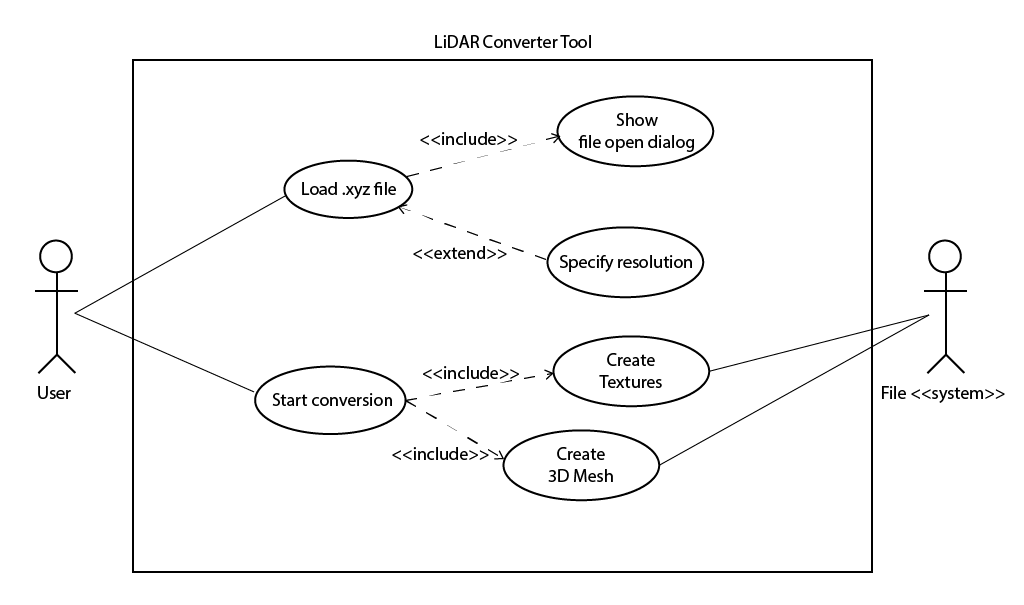
\includegraphics[scale=0.4]{UseCaseDiagram_PC2B.png}
	\caption{Use Case Diagram}
	\label{fig:use_case}
\end{figure}


\subsection{Laser scanning on location}

Cum sociis natoque penatibus et magnis dis parturient montes, nascetur ridiculus mus. Donec non auctor sem, sit amet fringilla purus. Phasellus eu orci et nibh lobortis faucibus id vel lorem. Aliquam ut diam id mi aliquam finibus eu id neque. Nam consequat efficitur mi sed maximus. Nullam egestas neque enim. Nulla nec eleifend mauris, eget sollicitudin velit. Quisque ultricies feugiat neque ut condimentum. Aliquam vehicula faucibus sapien non convallis. Nullam consectetur sagittis sollicitudin. Nulla mollis laoreet metus et consectetur.

\begin{figure}[h]
	\centering
	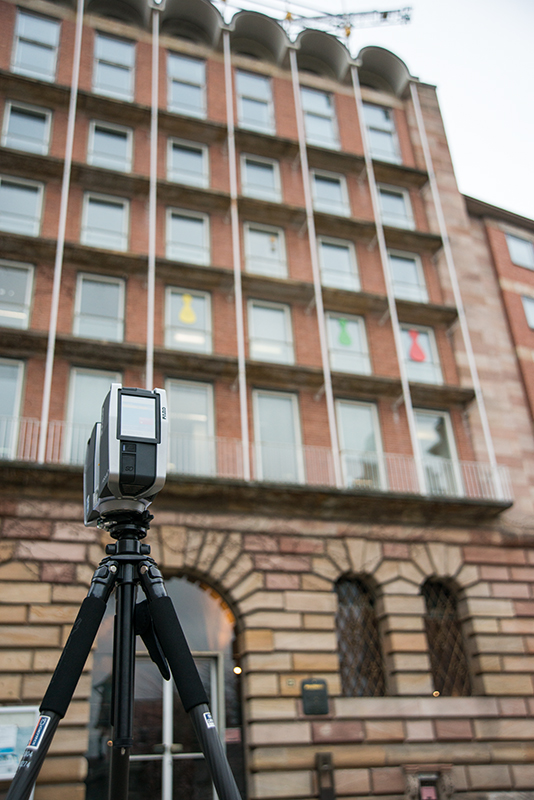
\includegraphics[scale=0.4]{PellerhausLaserScan.jpg}
	\caption{Scanning with Faro Focus 3D}
	\label{fig:laser_scanning_on_location}
\end{figure}



\begin{table}[h]
	\centering
	\begin{tabular}{l | l | l}
		A & B & C \\
		\hline
		1 & 3 & 4 \\
		1 & 3 & 4 \\
	\end{tabular}
	\caption{very basic table caption}
	\label{tab:abc}
\end{table}



\section{Generating data and testing algorithms}

\subsection{BlenSor}

Etiam non volutpat diam. Nam ac consectetur felis. Ut nec mi dictum, lobortis mauris quis, dapibus ligula. Nulla porttitor diam sed mauris dapibus posuere. Fusce pellentesque odio at nisl placerat porta. Donec urna risus, iaculis vitae justo quis, tempus ullamcorper diam. Integer eu gravida est. Phasellus eu ex tincidunt urna tempus pulvinar in in metus. Mauris tempus magna ac finibus suscipit. Praesent malesuada magna nibh, at rutrum felis semper a.

\subsection{Test-Addon for Blender}

Etiam non volutpat diam. Nam ac consectetur felis. Ut nec mi dictum, lobortis mauris quis, dapibus ligula. Nulla porttitor diam sed mauris dapibus posuere. Fusce pellentesque odio at nisl placerat porta. Donec urna risus, iaculis vitae justo quis, tempus ullamcorper diam. Integer eu gravida est. Phasellus eu ex tincidunt urna tempus pulvinar in in metus. Mauris tempus magna ac finibus suscipit. Praesent malesuada magna nibh, at rutrum felis semper a.

\section{Prototype}

\subsection{Point Cloud Importer}

Etiam non volutpat diam. Nam ac consectetur felis. Ut nec mi dictum, lobortis mauris quis, dapibus ligula. Nulla porttitor diam sed mauris dapibus posuere. Fusce pellentesque odio at nisl placerat porta. Donec urna risus, iaculis vitae justo quis, tempus ullamcorper diam. Integer eu gravida est. Phasellus eu ex tincidunt urna tempus pulvinar in in metus. Mauris tempus magna ac finibus suscipit. Praesent malesuada magna nibh, at rutrum felis semper a.

\subsubsection{Point Cloud data formats}

\begin{table}[h]
	\centering
	\begin{subtable}[h]{0.45\textwidth}
		\centering
		\begin{tabular}{l | l | l}
			Day & Max Temp & Min temp \\
			\hline \hline
			Mon & 20 & 13 \\
			Tue & 22 & 14 \\
			Wed & 23 & 12 \\
			Thu & 25 & 13 \\
			Fri & 18 & 7 \\
			Sat & 15 & 13 \\
			Sun & 20 & 13
		\end{tabular}
		\caption{First Week}
		\label{tab:week1}
	\end{subtable}
	\hfill
	\begin{subtable}[h]{0.45\textwidth}
		\centering
		\begin{tabular}{l | l | l}
			Day & Max Temp & Min Temp \\
			\hline \hline
			Mon & 17 & 11 \\
			Tue & 16 & 10 \\
			Wed & 14 & 8 \\
			Thu & 12 & 5 \\
			Fri & 15 & 7 \\
			Sat & 16 & 12 \\
			Sun & 15 & 9
		\end{tabular}
		\caption{Second Week}
		\label{tab:week2}
	\end{subtable}
	\caption{Max and min temp recorded during the first two weeks in January}
	\label{tab:temps}
\end{table}


\subsection{Projecting 3D points onto a 2D plane}

This is inside the text $\cos (2\theta) = \cos^2 \theta - \sin^2 \theta$.


And this is a separate formula:
$$\cos (2\theta) = \cos^2 \theta - \sin^2 \theta$$





\subsection{Saving textures}


\subsection{OpenGL Point Cloud Viewer}

This russian video tutorial was very helpful with the basic setup with the Qt framework.

\cite{ytQtOpenGL}

\subsection{Meshing}

Using the current pixel inside two for-loops in combination with the neighboring pixels to the right, bottom-right and bottom makes up a quad, which can be textured.

\subsection{Texture Coordinates and Normals}

Texture Coordinates go from 0.0 to 1.0 in the x and y direction, respectively. Usually the texture coordinate axes are referred to as s and t. By dividing the current coordinate by the width and the height of the image, respectively, the coordinates can be normalized.

Calculating normals is accomplished by using the cross product of the two vectors forming the current quad.

\subsection{Mesh Exporter}

There are different formats, one had to be chosen that supported at least vertices and faces.

\subsubsection{.obj}

The .obj format is the most popular and can be one of the easiest to understand file formats to save 3D geometry with not only points, but vertices, normals, texture coordinates and much more. It was the first choice when testing mesh exporting from the converter software and examining it in Blender.

\subsubsection{.blend}

A personal goal for this research was to implement a .blend export feature to allow for a native importing of the panorama mesh into Blender. However, this goal was not reached in this project. As it turned out, exporting the binary Blender file format was quite complicated, due to it's versatile structure. An experienced Blender Developer, Jeroen Bakker, stated in 2009 “When implementing loading and saving blend-files in a custom tool the difficulty is the opposite. In a custom tool loading a blend-file is easy, and saving a blend-file is difficult.” \parencite[see]{webMysteryOfTheBlend}. At least implementing it with the limited time for the thesis it was not feasable.



\subsubsection{custom format}

Even the Blender community suggested to not use the .blend format directly, but rather try a custom binary format. \parencite[compare]{webBlenderArtistsBlendExport}


\subsection{Optimizations}

The initial algorithms and approaches had some flaws, which needed to get eliminated to get a clean mesh out of the converter. Those are presented as follows:

\subsubsection{Flip horizontal direction of panorama}

The panorama is flipped horizontally.

\subsubsection{Panorama pixel depth testing}

It can happen that two points from the point cloud happen to result in the same pixel in the 2D panorama. This might result in a noisy image result, if not handled with care. To avoid any errors, it is important to take only the closest point to the camera, instead of letting every point override the corresponding pixel in the image.

\subsubsection{Panorama noise reduction}

Since there is only a limited number of points, the panorama texture gets quite noisy, especially with a higher resolution option set in the converter. A harsh change from light gray to black values in the depth map will result in a noisy 3D structure as well.
To solve this issue, the image is blurred by a user setting or automatically (TODO!).

\subsubsection{Remove doubles}

The meshing technique resulted in a very high point count for the .obj file. Example: For a 4x resolution panorama with 2,198,528 vertices, using the "remove doubles" option in Blender 3D automatically removed 2,100,716 vertices.
Solution: several passes for vertices, texture coordinates and normals (TODO!).

\subsubsection{3D Distortion}

The generated 3D mesh from the 2D panorama results in a distorted one, the more it touches the top.
Solution: None yet.

\subsubsection{Tiling}

Due to the higher resolution meshes having several megabytes in size and taking some time to import in Blender, this has to be optimized somehow.
Solution: Create tiles when higher resolution is set. E.g. with a 4x resolution, create four tiles (that's four seperate .obj files).
	\chapter{Production: Recreating the Pellerhaus from 1605}
	The generated mesh from PC2B may still need additional cleanup and detail. The mesh topology is dependend on the used meshing algorithm, naturally. It might not be ideal for an artist to have thousands of polygons build up a surface that could be represented by only one polygon. Furthermore the laser scanner beam cannot sample reflective or transparent structures, such as windows. Therefore it can only provide artists a great reference for manual tracing.

\section{Modeling the current Pellerhaus facade}

The lower part of the current Pellerhaus facade is very similar, almost identical, to the historic one. Thus modeling the modern facade based on LiDAR, photogrammetry and photographic reference appeared to make sense.

\subsection{Using the PC2B converter software}

Firstly, the LiDAR data was preprocesed in PC2B. We created five scans on location, so all the scans have been meshed with PC2B and imported into Blender. A manual registration of the scans was necessary in Blender, because the scans have been aquired at different locations. Fortunately, all the scans have been oriented similar due to the compass sensor in the laser scanner and the Pellerhaus facade was a good reference point to align them with each other.


It turned out that the workflow for artists is pretty much straight forward. Every scan took approximately 5 minutes to get processed by PC2B. Importing the result in Blender worked flawlessly and created all the necessary data blocks, like the named object and texture. We noticed that distinct names for the panorama textures need to be used to avoid multiple uses of one texture in different scans. The mesh is very helpful to get a sense of the scale of objects and where the detail is not sufficient, the texture information can help in finding details. Moreover, due to the clear texture the artist can select unnecessary polygons by simply choosing them from the image texture coordinates (which are usually called UV's in 3D applications) and delete them (see Chapter \ref{section_texture_coordinates_and_normals}). Other meshing algorithms, such as the Delaunay Tetrahedralization, create textures with very small UV islands and store them efficiently (see Appendix \ref{appendix_delaunay_texture_maps}).

All in all, PC2B generated a mesh that was helpful for tracing. This is how the imported scans look like in Blender:

\begin{figure}[h]
	\centering
	\includegraphics[width=1.0\textwidth]{Production_CombinedLaserScans.png}
	\caption{The manually registered LiDAR scans of the Pellerhaus}
	\label{fig:production_laser_scans_combined}
\end{figure}




\subsection{Using UAV references with photogrammetry}

Unmanned Aerial Vehicles (UAV's or simply drones) are getting affordable, even very good quality models. In our research we use the DJI Phantom 2 with a GoPro Hero 4 Black mounted on a 3-axis DJI Zenmuse H3-3D Gimbal to create photographic aerial references of the Pellerhaus Nürnberg.\\

Flying a drone legally is not as easy, as it might be assumed at first. Before even being able to take off with a UAV, German law requires a general permission for just entering the air space. In addition every UAV pilot needs an UAV insurance.\\

Regarding the usage of drones inside the city center of Nuremberg, there are more restrictions. The city center of Nuremberg is covered by the controlled air space. Flying in that air space is not permitted until the starting permission from the bavarian aviation authority and UAV insurance are upgraded to commercial ones. Furthermore pilots need a clearance from the Air traffic control (ATC). Additionally the starting and landing procedure requires to cordon off pedestrians and a special license from the traffic authority. Lastly, the owner of the property needs to be asked for permission to allow the starting and landing of the aircraft.\\

\pagebreak

Luckily there are some laws that permit video shoots and taking photos. For example the Freedom of panorama (§ 59, German Urheberrechtsgesetz) allows taking photos from pavements and roads permanently located in a public place. This right to freely take and share photographs of buildings and works of public art may be abolished on July 9th, 2015 by the European Parliament (see Blacker \parencite{freedomOfPanoramaUnderAttack}). We expect immense consequences for historic documentation of buildings if this happens.\\

In total we made three flights on location. It was planned to use the second flight for single photos shot in an interval of 1 second whereas the other two flights are videos in 4K. Unfortunately, it turned out that the third flight wasn't recorded at all and the second flight was captured as a video file. Luckily we noticed the third video missing while still on location, having a bit of battery life left and about one hour left to use the air space, so we made at least two impressive aerial shots before ending the mission.\\

With having video files instead of still images, those needed to be exported as still frames to be able to be processed by software. We tried both the free "Visual SfM" and commercial "Agisoft Photoscan Pro" software solutions to generate additional colored meshes of the Pellerhaus. The total processing time was about 20 hours for Visual SfM and 40 hours for Photoscan to get a 3D point cloud from the images. Comparing the results we noticed that Visual SfM generated a bend facade while Photoscan Pro kept it very straight. Although not recommended (compare Balletti et al. \parencite{calibration_of_action_cameras}), we used a GoPro camera with a short focal length and thus a strong lens distortion for 3d reconstruction. We can confirm, that the use of this camera is not a good choice, since the radial distortion can produce errors in the feature matching phase of photogrammetry. Still the output should be a good reference for the rough shape of the reconstructed object. If available, LiDAR data should be preferred over Photogrammetry for accurate building reconstruction.

\subsection{Using reference images}

In addition to the LiDAR data and Photogrammetry models, photos have been taken on location for additional reference. Very small details can be inspected in photographs while creating the surface to get them right. Based on the versatile data available, the model was built up slowly. First by creating the rough shapes for the building and constantly refining them to get the final model.

\pagebreak

\section{Modeling the historic Pellerhaus facade}

Based on the modern facade it was possible to get a good feel for the size of the Pellerhaus in the Renaissance. Still the main parts above the ground floor of the facade differ dramatically from the modern one. They can only be extracted from photographs.


\subsection{Using historic images as guide}

\begin{wrapfigure}{r}{0.5\textwidth}
	
	\centering
	
	\includegraphics[scale=0.1]{Production_Pellerhaus_1601_Entwurf_6.jpg}
	\hbox{\scriptsize Credit: Altstadtfreunde Nürnberg e.V.}
	\caption{Early draft of the Pellerhaus facade of around 1601}
	\label{fig:production_pellerhaus_draft}
	\vspace{-10pt}
	
\end{wrapfigure}

It is a huge luck that the Pellerhaus history has been documented by an enormous amount of pictures. A fascinating number of about 190 pictures has been provided for free through the association Altstadtfreunde Nürnberg e.V., not including about 100 additional pictures depicting the space in front of the building, to be used in this research.\\

This collection contains a few early drafts of the facade, likely created in the year 1601. Frontal, side or top views are best suited for modeling, especially when they are orthogonal (not distorted by perspective).\\

The modeling process began with adjusting the size of the image to the current Pellerhaus. The ground floor of the modern Pellerhaus was duplicated and served as the first guide for the creation of the upper floors. Floor by floor, bottom to top, was modelled by tracing the reference image (Figure \ref{fig:production_pellerhaus_draft}). This image was the clearest and best to work with to block out the historic facade shape. Unfortunately this was only possible to a certain degree. The Pellerhaus has a lot of tiny details, artistic ornaments and even sculptures at the top. These are so complex that the overall three-dimensional shape can only be estimated. Without historic experts it is very time-consuming to model the forms correctly. Due to this reason the historic model in this research only contains the obvious, rough forms of the facade. We hope that this model can be refined by working closely under the supervision of the association Altstadtfreunde Nürnberg e.V. in the future.

\subsection{Using historic stereoscopic images with photogrammetry}

Although the historic pictures have already been a blessing, there are two images aquired by stereophotography.


\begin{figure}[h]
	\centering
	\includegraphics[width=1.0\textwidth]{Production_Pellerhaus_1876_Stereo_Christian_Koenig_AF.jpg}
	\hbox{\scriptsize Credit: Christian König}
	\caption{Historic stereo pair from around 1876}
	\label{fig:production_stereo_historic}
\end{figure}


This project tried to extract the 3D information from those stereo pairs via photogrammetry. Feeding the left and right image into Agisoft Photoscan Pro, respectively, was expected to give a nice 3D representation of the historic facade. Unfortunately this did not work well:

\begin{figure}[h]
	\centering
	\begin{subfigure}[b]{0.45\textwidth}
		\centering
		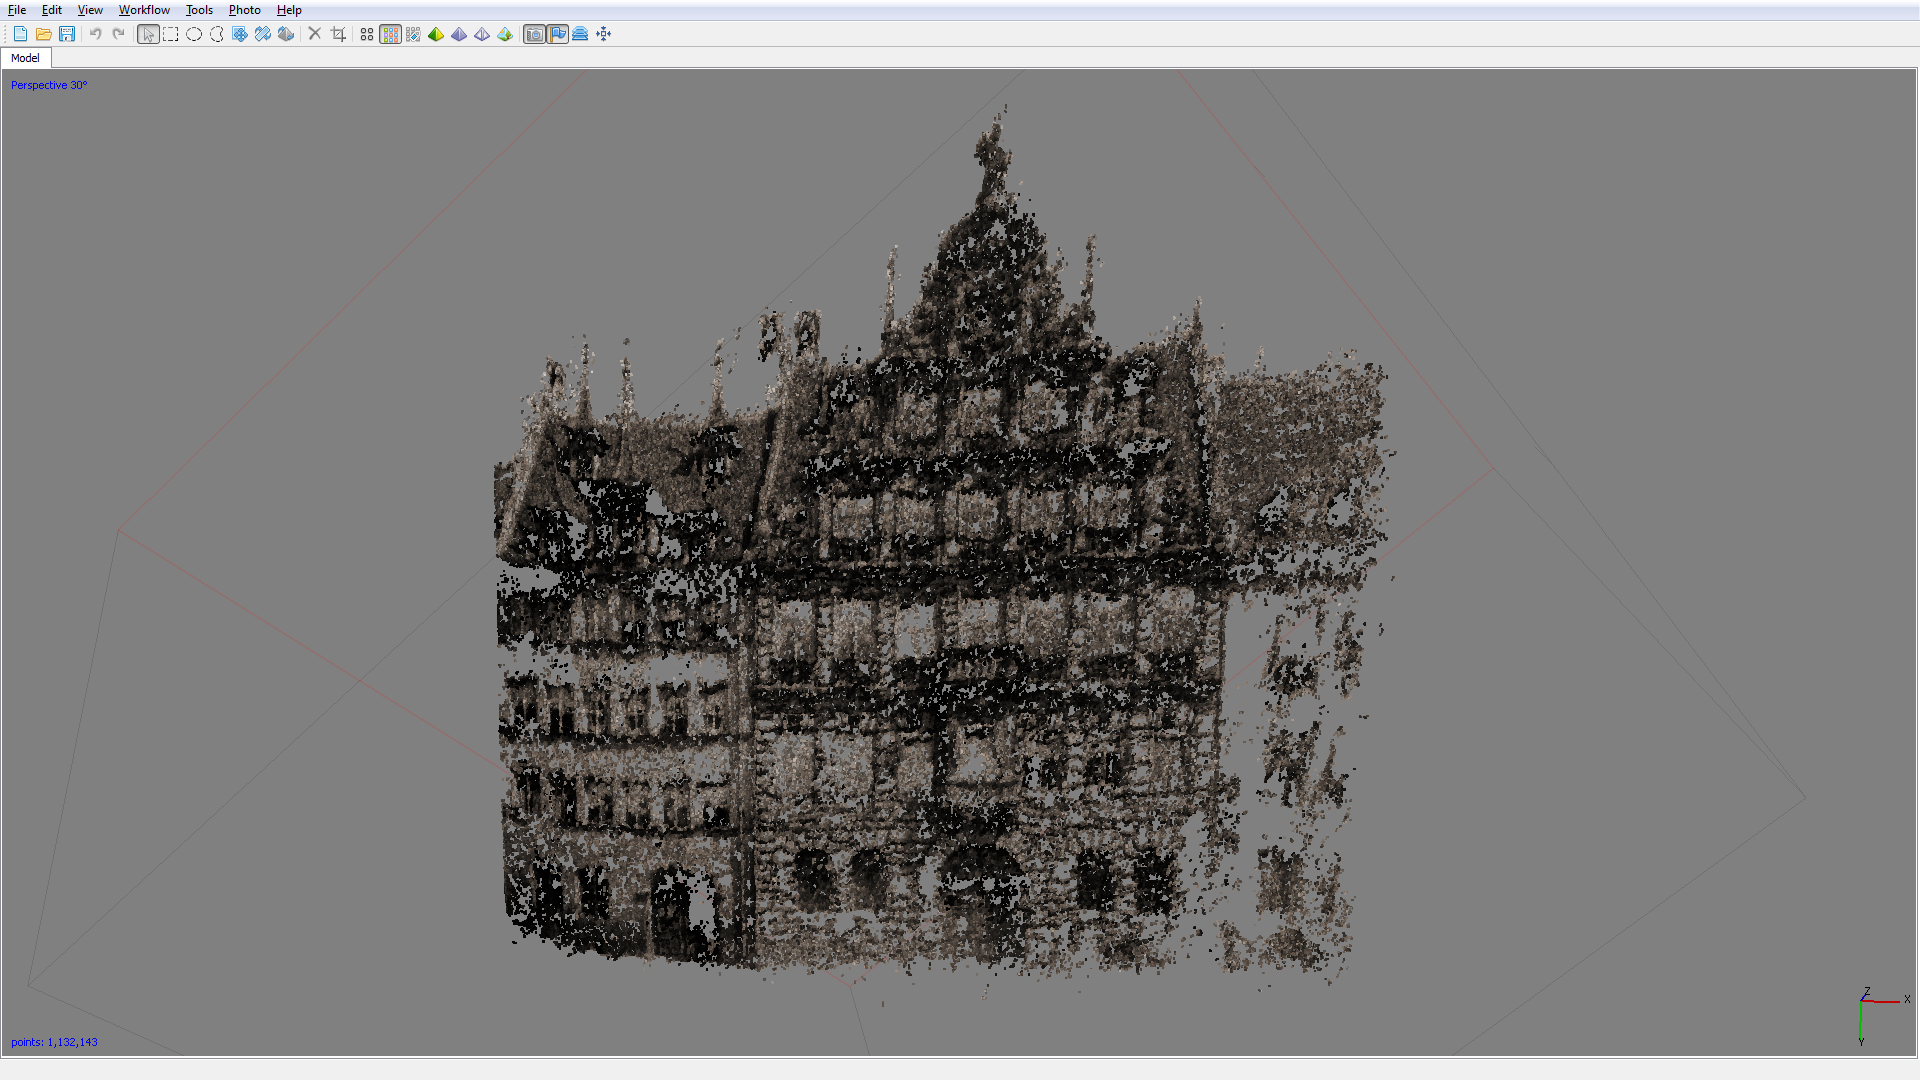
\includegraphics[width=\textwidth]{Production_StereoReconstruction_front.jpg}
		\caption{Historic point cloud front view}
		\label{fig:production_historic_stereo_reconstruction_front}
	\end{subfigure}
	\hfill
	\begin{subfigure}[b]{0.45\textwidth}
		\centering
		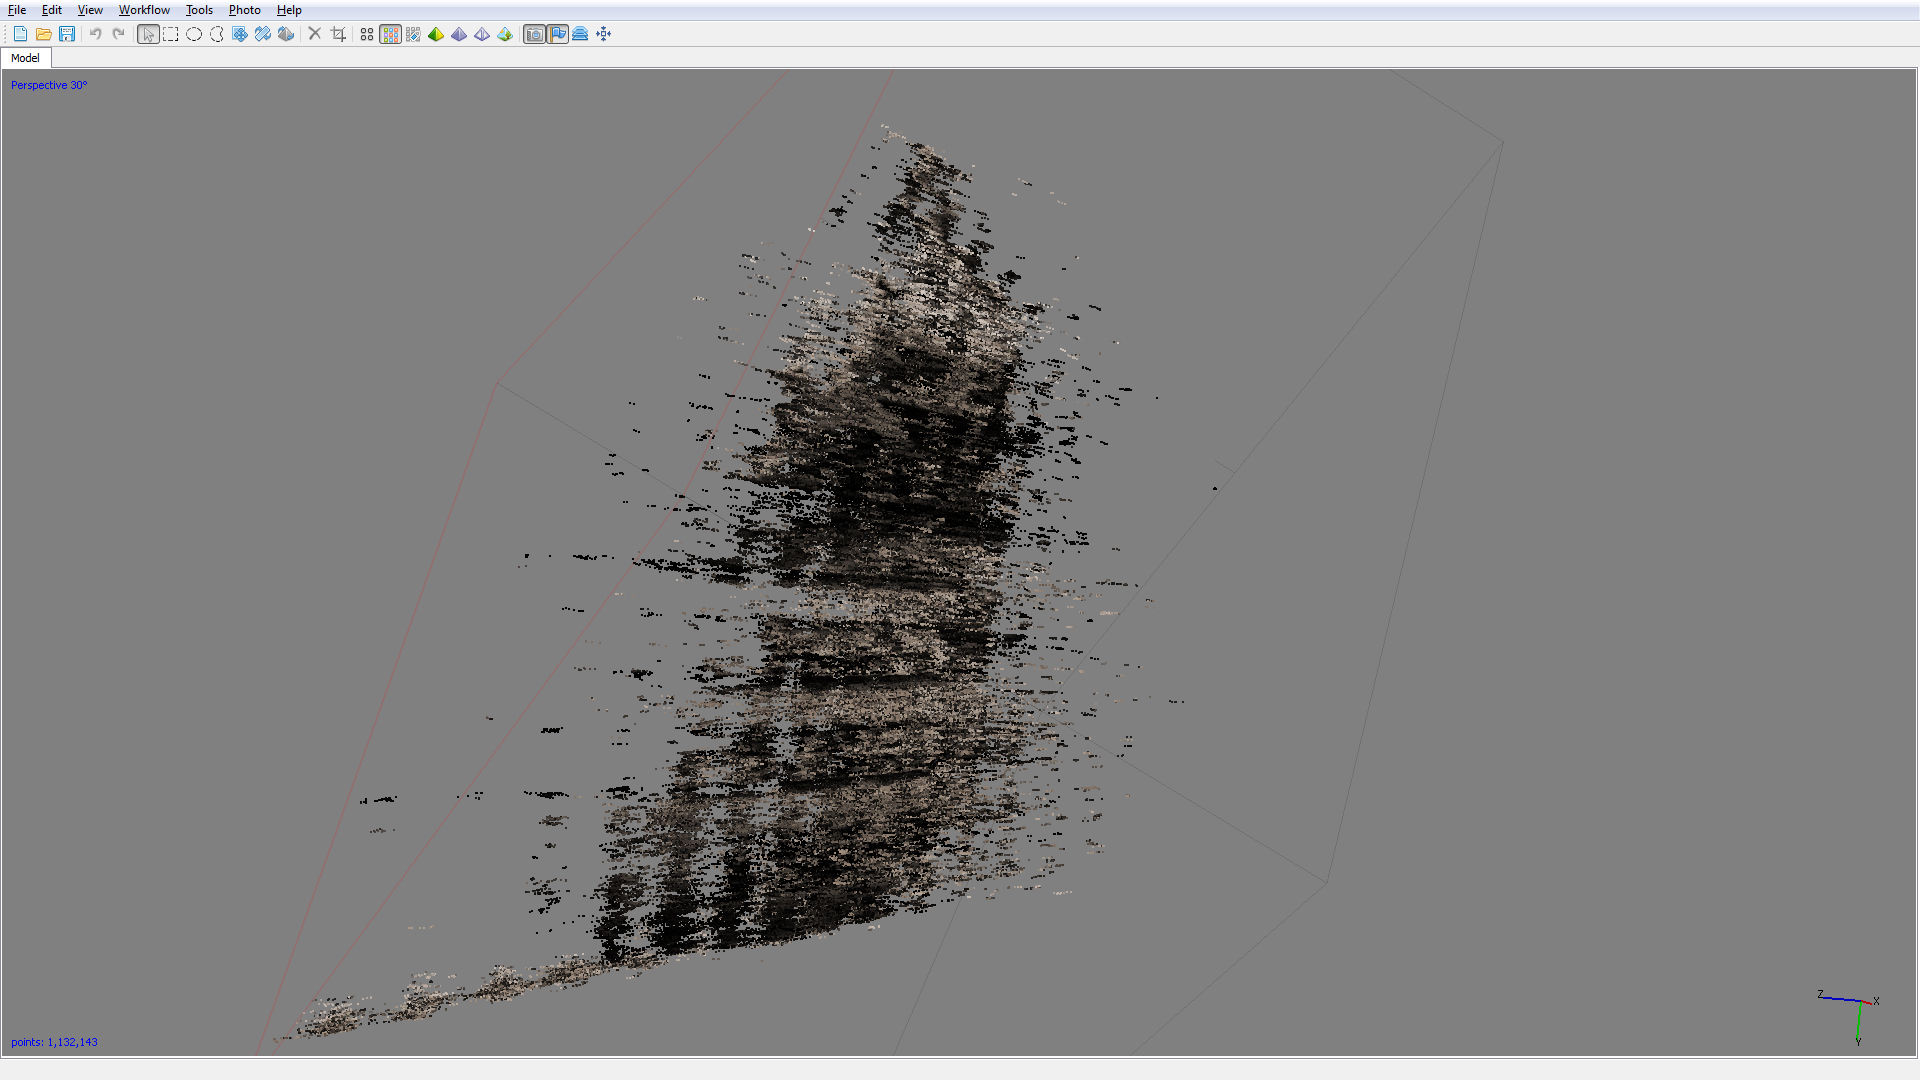
\includegraphics[width=\textwidth]{Production_StereoReconstruction_side.jpg}
		\caption{Historic point cloud right side view}
		\label{fig:production_historic_stereo_reconstruction_side}
	\end{subfigure}
	\caption{Automatic reconstruction results from historic stereo pairs}
	\label{fig:production_historic_stereo_reconstruction}
\end{figure}

The result is quite noisy, but might be suitable for a presentation if viewed carefully with only slight camera movements. However, the results are not satisfying in our view. Hence, they are not suited for the historic 3D reconstruction in this research.

\pagebreak

\section{The finished models}

The modeling process took 30 hours and 20 minutes to create the following results:

\begin{figure}[h]
	\centering
	\begin{subfigure}[b]{0.75\textwidth}
		\centering
		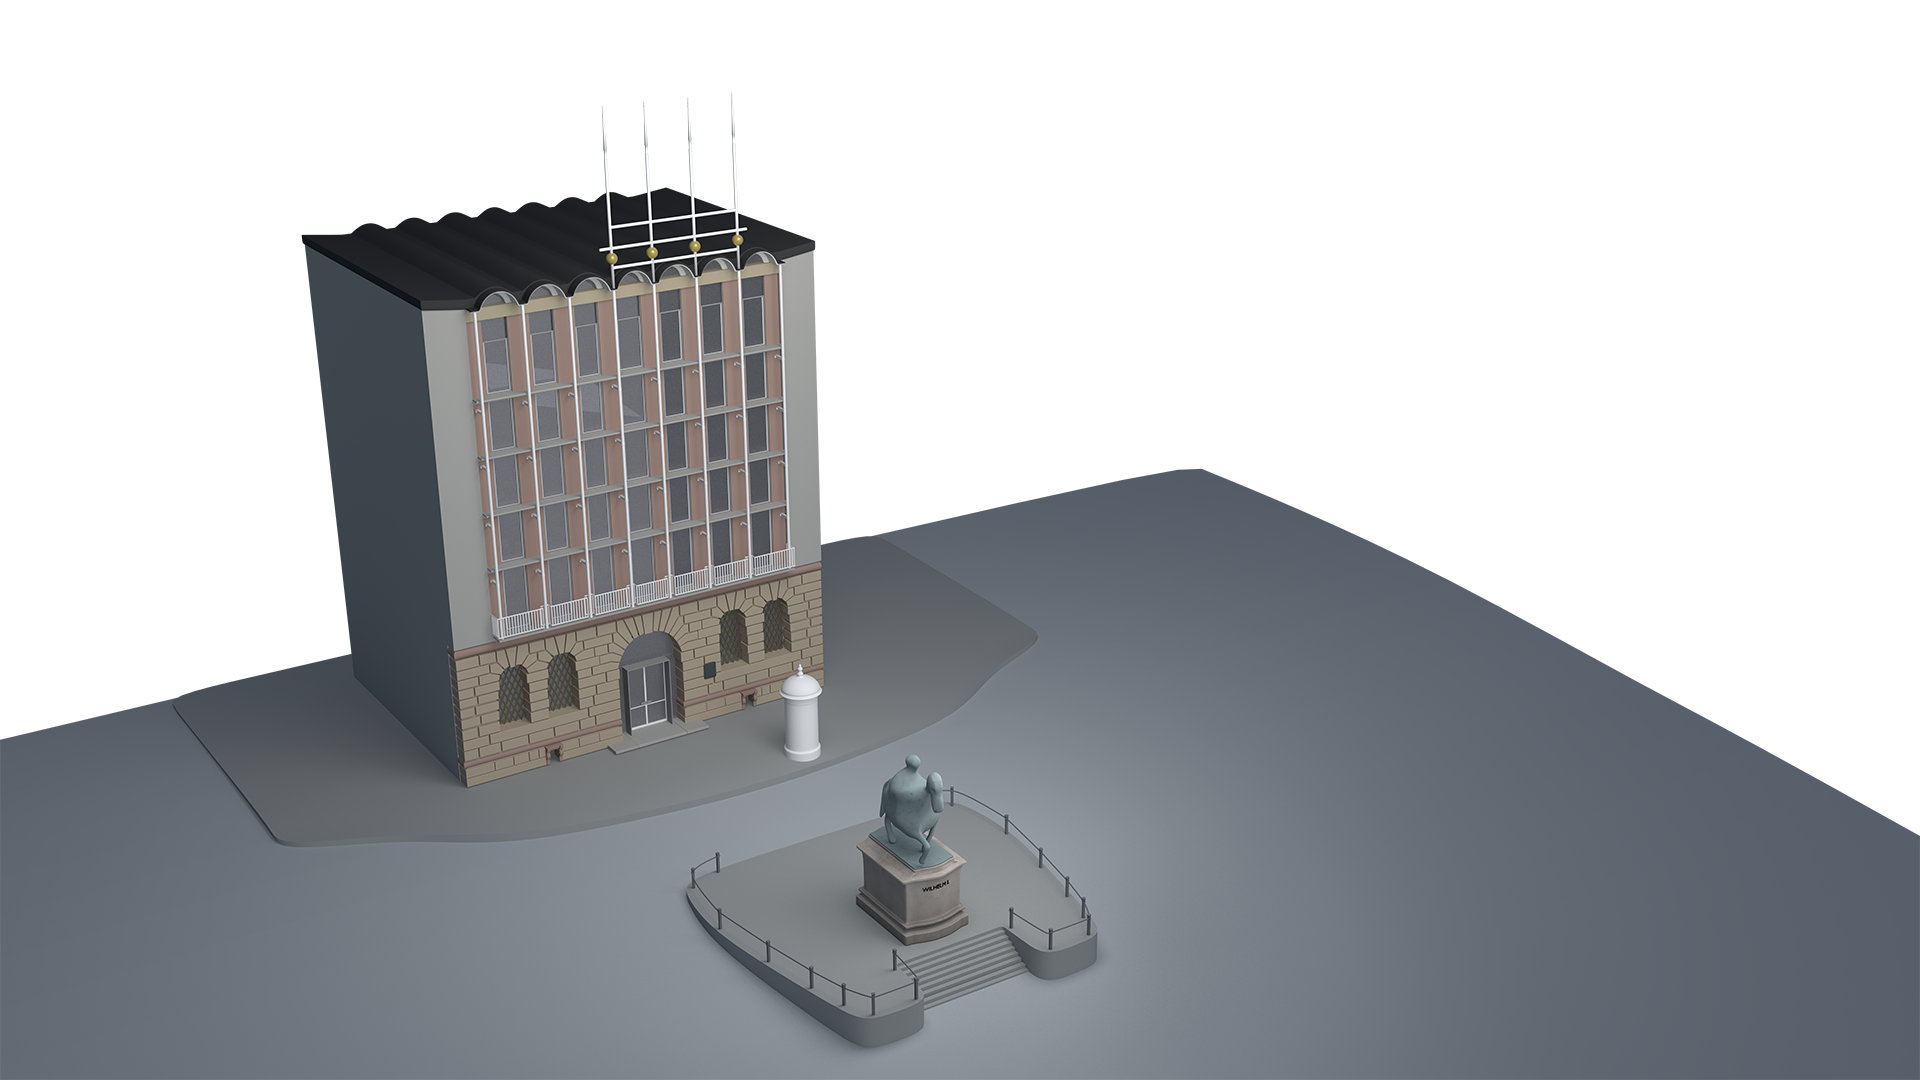
\includegraphics[width=\textwidth]{Pellerhaus_3d_a.png}
		\caption{Modern Pellerhaus}
		\label{fig:pellerhaus_3d_modern}
	\end{subfigure}
	\hfill
	\begin{subfigure}[b]{0.75\textwidth}
		\centering
		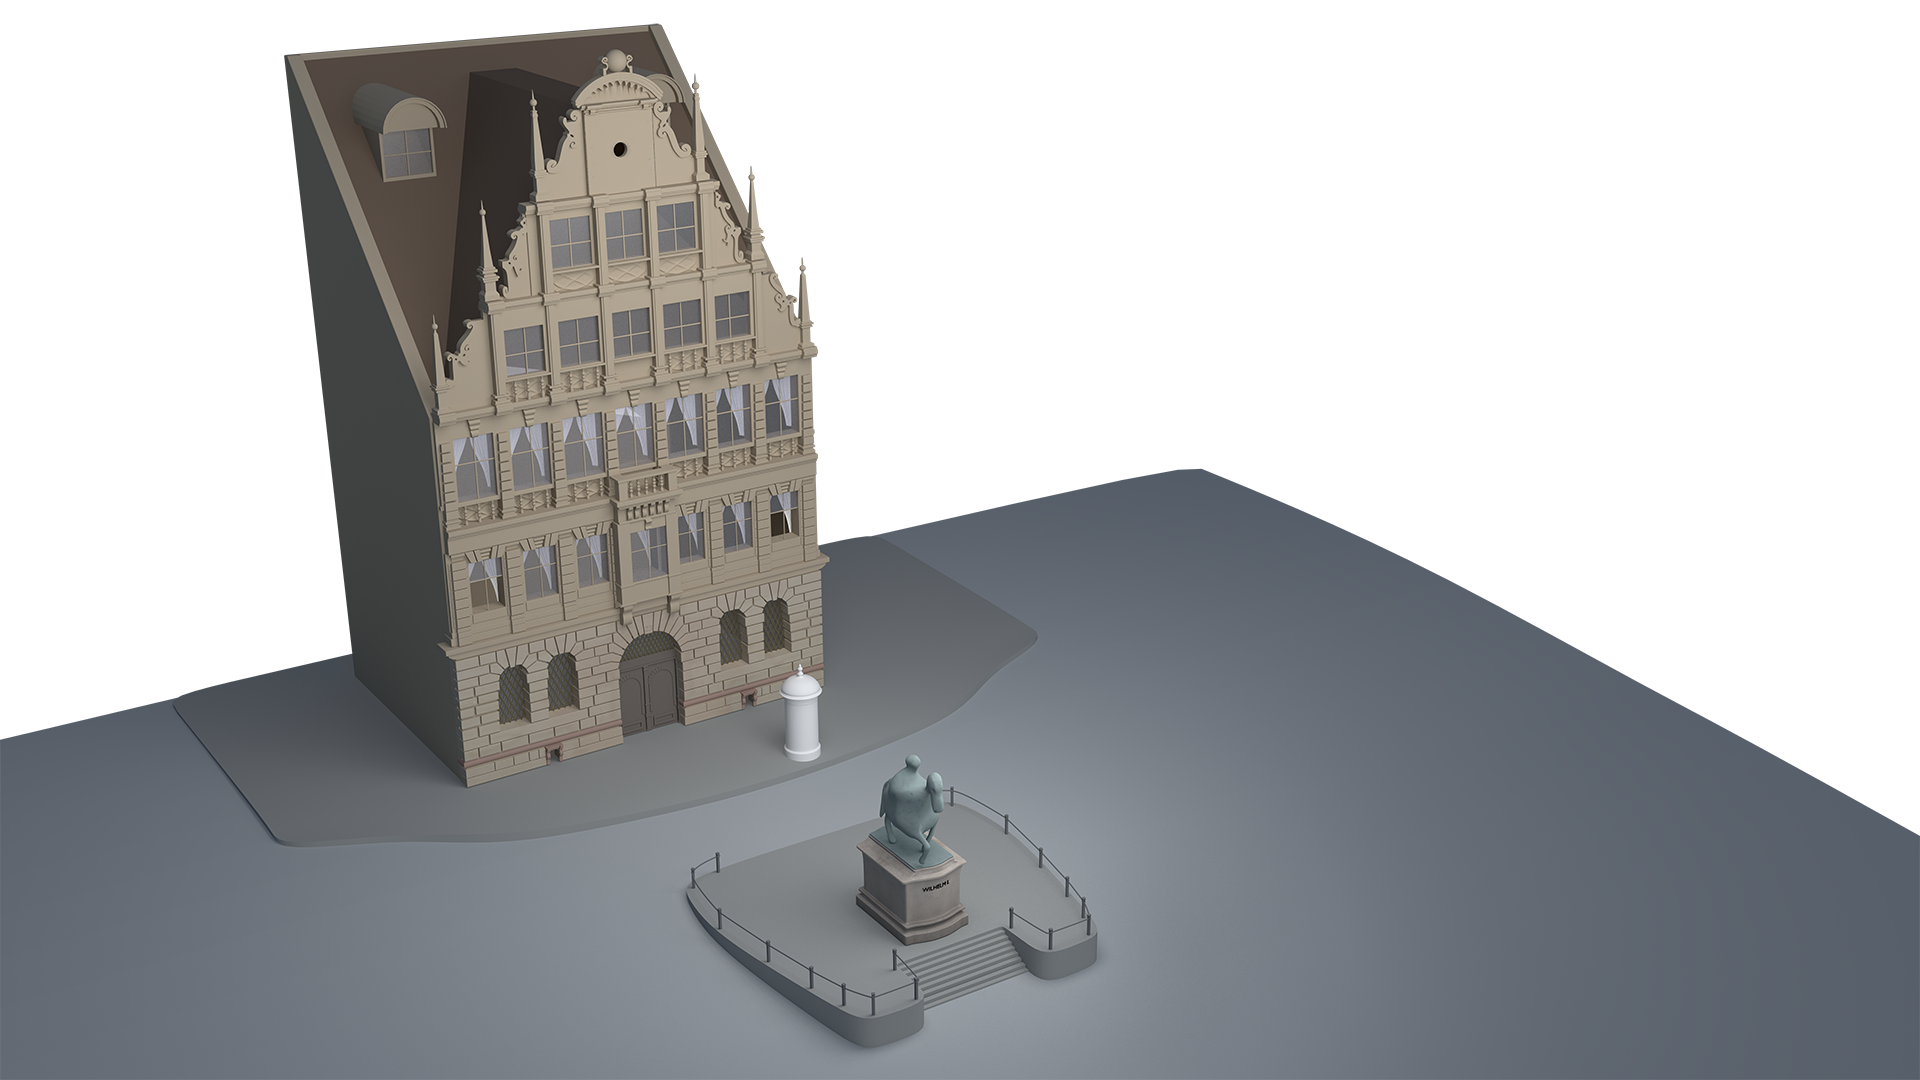
\includegraphics[width=\textwidth]{Pellerhaus_3d_b.png}
		\caption{Historic Pellerhaus}
		\label{fig:pellerhaus_3d_historic}
	\end{subfigure}
	\caption{The finished 3D models of the Pellerhaus}
	\label{fig:pellerhaus_3d_models}
\end{figure}

Rendering took 52 minutes for the modern building model and 54 minutes for the historic model. The render engine Cycles was used at a resolution of 7680 by 4320 pixels and 200 samples.\\

After refining the models, they can be animated to create educational videos about the Pellerhaus history. The historic Pellerhaus can be simulated to fracture and collapse during World War II only leaving debris and major parts of the ground floor. The debris can disappear slowly and the new facade will be created gradually. This may be supported visually by a timeline in the video. Finally, the finished video can be played out in stereoscopic 3D or the models can get 3D printed.\\

Timelapse videos have been created while modeling both buildings and will be published shortly after the research on the project website.

	\chapter{Conclusion and Future Work}
	\section{Conclusion}


Lorem ipsum dolor sit amet, consectetur adipiscing elit. Nullam hendrerit interdum sagittis. Nulla facilisi. Pellentesque laoreet tincidunt semper. Pellentesque pellentesque lectus id arcu interdum cursus ut ac dui. Etiam feugiat nisl ac odio suscipit pretium venenatis eget diam. Morbi molestie ipsum sit amet sapien rutrum luctus. Proin ac dolor ut metus laoreet aliquam non id nunc. Curabitur non efficitur dolor. Donec iaculis, dui et porta iaculis, magna tellus placerat ex, sed porta sem ligula ac augue. Fusce vitae sagittis ex. Pellentesque faucibus cursus elit, et faucibus velit cursus in. Nam lobortis id neque id hendrerit. Fusce et dolor nisi.

\section{Future Work}

Cum sociis natoque penatibus et magnis dis parturient montes, nascetur ridiculus mus. Donec non auctor sem, sit amet fringilla purus. Phasellus eu orci et nibh lobortis faucibus id vel lorem. Aliquam ut diam id mi aliquam finibus eu id neque. Nam consequat efficitur mi sed maximus. Nullam egestas neque enim. Nulla nec eleifend mauris, eget sollicitudin velit. Quisque ultricies feugiat neque ut condimentum. Aliquam vehicula faucibus sapien non convallis. Nullam consectetur sagittis sollicitudin. Nulla mollis laoreet metus et consectetur.

Etiam non volutpat diam. Nam ac consectetur felis. Ut nec mi dictum, lobortis mauris quis, dapibus ligula. Nulla porttitor diam sed mauris dapibus posuere. Fusce pellentesque odio at nisl placerat porta. Donec urna risus, iaculis vitae justo quis, tempus ullamcorper diam. Integer eu gravida est. Phasellus eu ex tincidunt urna tempus pulvinar in in metus. Mauris tempus magna ac finibus suscipit. Praesent malesuada magna nibh, at rutrum felis semper a.

Interdum et malesuada fames ac ante ipsum primis in faucibus. Cras quis pharetra libero. Pellentesque consectetur, quam vel ultrices finibus, sem enim consectetur mi, in dictum tellus leo eu ante. Maecenas consequat egestas erat, in vestibulum velit pulvinar ac. Suspendisse ullamcorper augue sapien, ac suscipit nulla dictum in. Nam sit amet congue ipsum. Aenean non felis malesuada, feugiat lectus a, tincidunt quam. Fusce nec quam egestas, vulputate est in, commodo nisi. Phasellus id nunc sit amet quam iaculis ornare eu id libero. Ut tempor nisi sed est pretium auctor. Donec in nunc turpis. Integer non tristique dolor. Curabitur a elit mollis urna finibus scelerisque sit amet vel erat. Nullam nec maximus erat. Duis ante mi, posuere ut lobortis nec, posuere eu ligula.

Aliquam at varius elit. Suspendisse viverra ex a ipsum scelerisque condimentum. Nam ac neque luctus, ullamcorper neque sit amet, tincidunt felis. Maecenas id orci rutrum, tincidunt nisl non, aliquam sapien. Aenean vestibulum erat ut nisl vehicula, quis rutrum eros fermentum. Maecenas ut arcu elit. Cras vestibulum pharetra facilisis. Quisque non elit iaculis leo dignissim faucibus. Etiam fringilla tortor nibh, sit amet volutpat diam consequat ac. Sed consectetur metus quis suscipit sollicitudin. Morbi imperdiet scelerisque nunc, in dapibus lacus. Praesent ullamcorper condimentum augue vitae finibus. 	
	
	
	\appendix
	\chapter{Appendix Title}
	\section{Software used}

\subsection{\LaTeX}
This paper was written in \LaTeX. On Windows, TeXstudio in conjunction with MikTeX (both portable versions) have been used for visual creation of the document. I decided to switch from the free version Adobe InDesign CS 2.0 to \LaTeX in favor of it being cross-platform and hoping to make it easier to publish the thesis online in the future. Since I have never worked with \LaTeX before, various tutorials \parencite{ytLaTeX,webLaTeX-Tutorial} on the internet have been a great help.

\subsection{Blender 3D}
To cleanup the generated mesh, retopologize it and create the 3D animations of the Pellerhaus, Blender was used.


\section{Programming libraries and frameworks}

\subsection{Qt 5.4}

Qt is an open source framework ...
	
	\printbibliography
		

\end{document}